% !TeX program = lualatex

\PassOptionsToPackage{ngerman}{babel}
\documentclass[
11pt, % The default document font size is 11 (recommended), options: 10pt, 11pt, 12pt
%oneside, % Two-side layout is recommended; uncomment to switch to one-sided
ngerman, % replace with ngerman for German; not fully supported so far -- requires changes elsewhere
singlespacing, % Single line spacing (recommended), alternatives: onehalfspacing or doublespacing
%draft, % Uncomment to enable draft mode (no pictures, no links, overfull hboxes indicated)
%nolistspacing, % If the document is onehalfspacing or doublespacing, uncomment this to set spacing in lists to single
%liststotoc, % Uncomment to add list of figures/tables/etc to table of contents (not recommended)
%toctotoc, % Uncomment to add the main table of contents to the table of contents (not recommended)
parskip, % add space between paragraphs (recommended)
nohyperref, % do not load the hyperref package (is loaded in setup.tex)
%headsepline, % print a horizontal line under the page header
consistentlayout, % layout of declaration, abstract and acknowledgements pages matches the default layout
%final, % Uncomment to hide all todo notes
]{PSIThesis} % The class file specifying the document structure

% version of the guide
\def\tversion{}

% long-term stable URL to the thesis guide
\def\doiurl{https://doi.org/10.20378/irb-48428}
\def\githuburl{https://github.com/UBA-PSI/psi-thesis-guide}

%%%%%%%%%%%%%%%%%%%%%%%%%%%%%%%%%%%%%%%%%%%%%%%%%%%
%
% File: setup.tex
%
% This file is part of the PSIThesis.cls
% LaTeX documentclass
%
% The code in this file is made available
% under the following license:
%
% LPPL v1.3c (http://www.latex-project.org/lppl)
%
%%%%%%%%%%%%%%%%%%%%%%%%%%%%%%%%%%%%%%%%%%%%%%%%%%%


%----------------------------------------------------------------------------------------
%		UNIVERSITY OF BAMBERG COLORS
%----------------------------------------------------------------------------------------

% http://www.brandwares.com/RGBTintCalculator.php
% Base Color value obtained from UB Corporate Identity Manual
\definecolor{ubblue}{HTML}{00457D}
\definecolor{ubblue80}{HTML}{336A97}
\definecolor{ubblue60}{HTML}{668FB1}
\definecolor{ubblue40}{HTML}{99B5CB}
\definecolor{ubblue20}{HTML}{CCDAE5}

\definecolor{ubyellow}{HTML}{FFD300}
\definecolor{ubyellow25}{HTML}{FFF4BF}

\definecolor{ubred}{HTML}{e6444F}

\definecolor{ubgreen}{HTML}{97BF0D}

\definecolor{gray75}{gray}{0.75}
\definecolor{gray50}{gray}{0.50}

%----------------------------------------------------------------------------------------
%		FONT SETUP
%----------------------------------------------------------------------------------------

%\usepackage[T1]{fontenc} % Output font encoding for international characters - do not use T1 encoding with luatex!
\usepackage[utf8]{luainputenc} % makes unicode characters like –, €, and ß work properly

% amssymb must be loaded before newtxmath to avoid this error:
% Command `\Bbbk' already defined
\usepackage{amssymb}
\usepackage[cochineal]{newtxmath} % must be loaded before fontspec

\usepackage[no-math]{fontspec} % allows us to use OTF/TTF fonts, but do not interfere with math (because we use newtxmath, which does support Cochineal)

% If you cannot use the cochineal font, uncomment the following lines to select
% the Crimson font. Note, however, that you'll have to take care of the math font
% on your own.
%
%\setmainfont[
%	Path           = fonts/,
%    BoldFont       = {Crimson-Semibold.otf},
%    ItalicFont     = {Crimson-Italic.otf},
%    BoldItalicFont = {Crimson-BoldItalic.otf}
%]{Crimson-Roman.otf}

\setmainfont{Cochineal}[
  Numbers={Proportional,OldStyle},
  Style=Swash % for nice swashed Q letter, see https://golatex.de/spezeielle-opentype-features-in-fontspec-aktivieren-t19831.html
]
%\setmainlanguage{english}
\DeclareSymbolFont{operators}{\encodingdefault}{\familydefault}{m}{n} %  render numbers in cochineal, cf. https://tex.stackexchange.com/questions/398895/using-two-different-math-fonts-with-lualatex

% imitate the behavior of the cochineal package as follows:
% cf. https://tex.stackexchange.com/questions/448895/fontenc-vs-fontspec-with-xelatex
\DeclareRobustCommand{\lfstyle}{\addfontfeatures{Numbers=Lining}}
\DeclareTextFontCommand{\textlf}{\lfstyle}
\DeclareRobustCommand{\tlfstyle}{\addfontfeatures{Numbers={Tabular,Lining}}}
\DeclareTextFontCommand{\texttlf}{\tlfstyle}

% Exception: tables should use "lining figures" (all digits having same width)
\AtBeginEnvironment{tabular}{%
  \tlfstyle
}
\AtBeginEnvironment{tabularx}{%
  \tlfstyle
}


% monospace font, will be used in verbatim and listing environments
\setmonofont[
	Path           = fonts/,
    BoldFont       = {iosevka-ss04-bold.ttf},
    ItalicFont       = {iosevka-ss04-italic.ttf},
    BoldItalicFont       = {iosevka-ss04-bolditalic.ttf},
    Scale = 0.83 % manually determined value;
]{iosevka-ss04-regular.ttf}


% sans-serif font, will be used in the margins
\setsansfont[
	Path          	= fonts/,
	BoldFont		= Roboto-Bold.otf,
	ItalicFont		= Roboto-Italic.otf,
	BoldItalicFont	= Roboto-BoldItalic.otf,
	Scale = 0.83 % manually determined value;
]{Roboto-Regular.otf}

\renewcommand{\familydefault}{\rmdefault}
\defaultfontfeatures{Ligatures=TeX}


%----------------------------------------------------------------------------------------
%		HEADINGS SETUP (CHAPTERS, SECTIONS, …)
%----------------------------------------------------------------------------------------

\usepackage[explicit]{titlesec}
\newcommand{\hsp}{\hspace{20pt}}

\setcounter{secnumdepth}{3}

% We use lining figures for headers (tlfstyle) because they fit better with uppercase letters than old-style figures.

% chapters have a vertical line between number and title
\titleformat{\chapter}[hang]{\Huge\bfseries\tlfstyle}{\color{black}\thechapter}{20pt}{\begin{tabular}[t]{@{\color{ubblue60}\vrule width 2pt\hsp}p{0.85\textwidth}}\raggedright #1\end{tabular}}

% sections
\titleformat{\section}[hang]{\bfseries\large\tlfstyle}{{\color{ubblue}\thechapter.\arabic{section}}}{1ex}{{\color{ubblue} #1}}{}

% subsections
\titleformat{\subsection}[hang]{\bfseries\large\tlfstyle}{{\color{ubblue}\thechapter.\arabic{section}.\arabic{subsection}}}{1ex}{{\color{ubblue} #1}}{}

% subsubsections
\titleformat{\subsubsection}[hang]{\bfseries\tlfstyle}{{\color{ubblue}\thechapter.\arabic{section}.\arabic{subsection}.\arabic{subsubsection}}}{1ex}{{\color{ubblue} #1}}{}

% vertical spacing for headings ==============
\titlespacing*{\section}
{0pt}{7ex}{3ex}

\titlespacing*{\subsection}
{0pt}{4ex}{2ex}

\titlespacing*{\subsubsection}
{0pt}{4ex}{2ex}
% end of vertical spacing ====================

%----------------------------------------------------------------------------------------
%		TABLE OF CONTENTS SETUP
%----------------------------------------------------------------------------------------

% solution inspired from https://tex.stackexchange.com/questions/178510/how-can-i-reproduce-this-beautiful-table-of-contents
\usepackage{etoc}
\etocsetlevel{section}{2}
\etocsetlevel{subsection}{3}

\etocsettocdepth{section} % set to subsection for adding subsections to toc (not recommended)

\newlength{\tocleft}
\setlength{\tocleft}{2.5cm} % must be set to fit the innermargin defined in geometry (change only if you have changed the margins)

\newlength{\tocsep}
\setlength{\tocsep}{2em}

\usepackage{textcase}


\etocsetstyle{chapter}
   {}
   {}
   {\etocifnumbered
     {\makebox[0pt][r]
       % we use \etocthenumber instead of \etocnumber to avoid the href, which is part of \etocthenumber, messing with MakeTextLowercase
       {\textsc{\MakeTextLowercase\chaptername\ \MakeTextLowercase\etocthenumber}\hspace{\tocsep}}%
       \textbf{\etocname\kern1em\relax\etocpage}%
    }%
    {\textbf{\etocname\kern1em\relax\etocpage}}%
    \par\vspace{3ex}%
   }%
   {}

\etocsetstyle{section}
   {\vspace{-2ex}} % Muss von den 3ex aus Chapter abgezogen werden
   {}
   % see the comment regarding etocthenumber in the chapter style definition
   {\makebox[0pt][r]{\textsc{\MakeTextLowercase\etocthenumber}\hspace{\tocsep}}%
    \etocname\kern1em\etocpage\par%
   }%
   {\addvspace{3ex}} % 3ex falls danach Chapter kommt

\etocsetstyle{subsection}
   {\vspace{0ex}}
   {}
   {\makebox[3em][l]{\etocnumber}\etocname\kern1em\etocpage\par}
   {\addvspace{2ex}} % 2ex falls danach Section kommt

\etocsettocstyle{\chapter*{\contentsname}
                \thispagestyle{plain}%
                \leftskip\tocleft\parindent0pt}{}


%----------------------------------------------------------------------------------------
%		OTHER PACKAGES
%----------------------------------------------------------------------------------------
\usepackage{acronym} % for abbreviations
\usepackage{tabularx} % for more flexible tables

\usepackage{marginnote} % Enable Notes on the Page Margin
\usepackage{marginfix} % Enables floating for margin figures
\usepackage{ragged2e} % provides better hyphenation, use with camel case: \RaggedRight
\renewcommand*{\raggedleftmarginnote}{\RaggedLeft}
\renewcommand*{\raggedrightmarginnote}{\RaggedRight}

% justified margin notes:
% uncomment the following two lines to for justified layout of margin notes
%\renewcommand*{\raggedleftmarginnote}{\RaggedLeft}
%\renewcommand*{\raggedrightmarginnote}{\RaggedRight}



\renewcommand*{\marginfont}{\setlength{\parskip}{0.5ex}\scriptsize\sffamily} % format margin text



% for sidenotes: change marginpar font
\usepackage{xparse}
\let\oldmarginpar\marginpar
\RenewDocumentCommand{\marginpar}{om}{%
  \IfNoValueTF{#1}
    {\oldmarginpar{\mymparsetup #2}}
    {\oldmarginpar[\mymparsetup #1]{\mymparsetup #2}}}
\newcommand{\mymparsetup}{\scriptsize\sffamily}


% this provides correct alignment for margin text that is inserted
% right at the beginning of a paragraph; however, it messes up the
% alignment in all other cases.
%% therefore, removed for now:
%%\renewcommand{\marginnotevadjust}{0.71\baselineskip}
% The following is the necessary correction for in-paragraph use
\renewcommand{\marginnotevadjust}{0.21\baselineskip}
\renewcommand{\marginnotevadjust}{0.55\baselineskip}

\usepackage{microtype} % enable better typographic setup

\usepackage{multicol} % enable usage of multiple columns

% biblatex setup
% inspired by https://anneurai.net/2017/10/18/thesis-formatting-in-latex/
\usepackage[
  backend=biber,
  style=alphabetic,
  doi=false,isbn=false, % these fields are commonly omitted
  terseinits=true, % no points between initials
  giveninits=true, % always print only initials for given names
  sortcites=true,
  language=english,
  backref=true, % show on what pages a ref has been cited
]{biblatex} % Use biber backend with alphabetic reference style
\AtEveryBibitem{%
  \clearlist{language} % don't show "en."
  \clearlist{extra} % clears extra fields such as ISBN nrs
}

% shorten the strings used in back references
\DefineBibliographyStrings{english}{%
  backrefpage = {page},
  backrefpages = {pages},
}

%-- no "quotes" around titles of chapters/article titles
\DeclareFieldFormat[article, inbook, incollection, inproceedings, misc, thesis, unpublished]{title}{#1}
%-- no punctuation after volume
\DeclareFieldFormat[article]{volume}{{#1}}
%-- puts number/issue between brackets
\DeclareFieldFormat[article, inbook, incollection, inproceedings, misc, thesis, unpublished]{number}{\mkbibparens{#1}}
%-- and then for articles directly the pages w/o any "pages" or "pp."
\DeclareFieldFormat[article]{pages}{#1}
%-- format 16(4):224--225 for articles
\renewbibmacro*{volume+number+eid}{\printfield{volume}\printfield{number}\printunit{\addcolon}
}
\DeclareFieldFormat{url}{\url{#1}}


\usepackage[autostyle=true]{csquotes} % Required to generate language-dependent quotes in the bibliography

\usepackage[
  obeyFinal,
  textsize=scriptsize,
  backgroundcolor=ubyellow25,linecolor=ubyellow,bordercolor=ubyellow,
]{todonotes}

% change font of todo notes to sans-serif
\makeatletter
\renewcommand{\todo}[2][]{\@bsphack\@todo[#1]{\sffamily #2}\@esphack\ignorespaces}
\makeatother

\usepackage{booktabs} % use formal table layout

\urlstyle{same} % avoids printing URLs in typewriter font

% enable very extensive URL breaking
% https://tex.stackexchange.com/questions/3033/forcing-linebreaks-in-url
\PassOptionsToPackage{hyphens}{url}
\expandafter\def\expandafter\UrlBreaks\expandafter{\UrlBreaks% save the current one
  \do\a\do\b\do\c\do\d\do\e\do\f\do\g\do\h\do\i\do\j%
  \do\k\do\l\do\m\do\n\do\o\do\p\do\q\do\r\do\s\do\t%
  \do\u\do\v\do\w\do\x\do\y\do\z\do\A\do\B\do\C\do\D%
  \do\E\do\F\do\G\do\H\do\I\do\J\do\K\do\L\do\M\do\N%
  \do\O\do\P\do\Q\do\R\do\S\do\T\do\U\do\V\do\W\do\X%
  \do\Y\do\Z\do\*\do\-\do\~\do\'\do\"\do\-}%

% TODO consider using package xurl, which is supposed to handle url breaking

% https://tex.stackexchange.com/a/450695
% allow URLs to be spaced out at / => much better URL breaking in margins
\makeatletter
\g@addto@macro\UrlSpecials
{%
    \do\/{\mbox{\UrlFont/}\hskip 0pt plus 0.1em minus 0.1em}%
}
\Urlmuskip=0mu plus 1mu\relax
\makeatother


% hyperlink layout
\usepackage{hyperref}
 \hypersetup{colorlinks,breaklinks,unicode,
             citecolor=ubblue60,
             linkcolor=ubblue60,
             filecolor=ubblue60,
             urlcolor=ubblue60}

% cleverref allows you to use \Cref{sec:foo} to get the text "Section 1.2".
% This also works with figures and tables.
\usepackage{cleveref}

% datetime is use to automatically handle the date rendering on the titlepage.
\usepackage{datetime}
% rendering the current date as Month/JJJJ
% see: https://tex.stackexchange.com/questions/212263/month-year-format-in-latex
\newdateformat{monthyeardate}{%
  \monthname[\THEMONTH] \THEYEAR}


\raggedbottom % do NOT force all pages to have the same height (which would be done by increasing the space between paragraphs, which can create noisy layouts)

%----------------------------------------------------------------------------------------
%	SETUP BIBLIOGRAPHY
%----------------------------------------------------------------------------------------
\setlength{\bibitemsep}{.3\baselineskip plus .05\baselineskip minus .05\baselineskip}
\newlength{\bibparskip}\setlength{\bibparskip}{0pt}
\let\oldthebibliography\thebibliography
\renewcommand\thebibliography[1]{%
  \oldthebibliography{#1}%
  \setlength{\parskip}{\bibitemsep}%
  \setlength{\itemsep}{\bibparskip}%
}

% allow much more liberal line breaks in URLs
\setcounter{biburllcpenalty}{7000}
\setcounter{biburlucpenalty}{8000}

% adjust space between key and entry, default is 2\labelsep
\setlength{\biblabelsep}{1\labelsep}

% configures indentation of bibentries
\defbibenvironment{bibliography}
  {\list
     {\hspace{0.5\labelalphawidth}\bfseries\printtext[labelalphawidth]{%
        \printfield{prefixnumber}%
        \printfield{labelalpha}%
        \printfield{extraalpha}}}
     {\setlength{\labelsep}{\biblabelsep}%
      \setlength{\leftmargin}{0.5\labelalphawidth}%
      \setlength{\itemsep}{1.5\bibitemsep}%
      \setlength{\parsep}{\bibparsep}}%
      \renewcommand*{\makelabel}[1]{##1\hss}}
  {\endlist}
  {\item}


%----------------------------------------------------------------------------------------
%	MARGIN SETTINGS
%----------------------------------------------------------------------------------------

% Using the layout from kaobook
\geometry{
		paper=a4paper,
		head=13.6pt,
		top=27.4mm,
		bottom=27.4mm,
		inner=24.8mm,
		%outer=24.8mm,
		%right=2.183cm,
		textwidth=107mm,
		marginparsep=8.2mm,
		marginparwidth=49.4mm,
		%textheight=49\baselineskip,
		includemp,
		% showframe
}

% Wide figures span text and margin.
% Use the pre-calculated length \widefigurewidth in \includegraphics.
\def\widefigurewidth{\dimexpr(\marginparwidth + \textwidth + \marginparsep)}


%----------------------------------------------------------------------------------------
%	SETUP HEADER AND FOOTER
%----------------------------------------------------------------------------------------


\newlength{\overflowingheadlen}
\setlength{\overflowingheadlen}{\textwidth}
\addtolength{\overflowingheadlen}{\marginparsep}
\addtolength{\overflowingheadlen}{\marginparwidth}

% old header/footer, maybe not necessary any more?
\automark[chapter]{chapter}
\ihead{\textup{\headmark}} % Inner header; do not use italics: therefore textup
\ihead{\textup{\textsc{\MakeLowercase\headmark}}}% Inner header - use this line for Small Caps in header
\ohead[]{\pagemark} % Outer header
\cfoot[\pagemark]{} % On chapter opening pages, the page number goes centered into the footer
\automark*[section]{}%

% new header/footer, from kaobook; we could probably remove the original definitions from the cls
\renewpagestyle{thesis}{
  {\hspace{-\marginparwidth}\hspace{-\marginparsep}\makebox[\overflowingheadlen][l]{\textup{\thepage}\quad\rule[-\dp\strutbox]{1pt}{\baselineskip}\quad{}\textup{\textsc{\MakeLowercase \leftmark}}}}%
  {\makebox[\overflowingheadlen][r]{\textup{\textsc{\MakeLowercase \rightmark}}\quad\rule[-\dp\strutbox]{1pt}{\baselineskip}\quad\textup{\thepage}}}%
  {}
}{
  {}%
  {}%
  {}
}
\renewpagestyle{plain.thesis}{
  {}%
  {}%
  {}
}{
  {\hspace{-\marginparwidth}\hspace{-\marginparsep}\makebox[\overflowingheadlen][l]{\textup{\textsc{\thepage}}\quad\rule[-\dp\strutbox]{1pt}{\baselineskip}}}%
  {\makebox[\overflowingheadlen][r]{\rule[-\dp\strutbox]{1pt}{\baselineskip}\quad\textup{\textsc{\thepage}}}}%
  {}
}

%----------------------------------------------------------------------------------------
%	LISTINGS SETTINGS
%----------------------------------------------------------------------------------------

\usepackage{textcomp}
\usepackage{listings}
\definecolor{darkgray}{rgb}{.4,.4,.4}

\lstdefinelanguage{JavaScript}{
  keywords={typeof, new, true, false, catch, function, return, null, catch, switch, var, if, in, while, do, else, case, break},
  ndkeywords={class, export, boolean, throw, implements, import, this},
  sensitive=false,
  comment=[l]{//},
  morecomment=[s]{/*}{*/},
  morestring=[b]',
  morestring=[b]"
}

\lstset{
    aboveskip={1\baselineskip},
    abovecaptionskip=-1\baselineskip,
    belowcaptionskip=2ex,
    basicstyle=\footnotesize\ttfamily\linespread{4},
    breaklines=true,
    columns=flexible,
    commentstyle=\color{gray50}\ttfamily\itshape,
    escapechar=@,
    extendedchars=true,
    frame=l,
    framerule=.5pt,
    identifierstyle=\color{black},
    inputencoding=latin1,
    keywordstyle=\color{ubblue80}\bfseries,
    ndkeywordstyle=\color{ubblue80}\bfseries,
    numbers=left,
    numbersep=1.25em,
    numberstyle=\scriptsize\ttfamily,
    prebreak = \raisebox{0ex}[0ex][0ex]{\ensuremath{\hookleftarrow}},
    stringstyle=\color{ubblue60}\ttfamily,
    upquote=true,
    showstringspaces=false,
}

\lstset{literate=%
   *{0}{{{\color{darkgray}0}}}1
    {1}{{{\color{darkgray}1}}}1
    {2}{{{\color{darkgray}2}}}1
    {3}{{{\color{darkgray}3}}}1
    {4}{{{\color{darkgray}4}}}1
    {5}{{{\color{darkgray}5}}}1
    {6}{{{\color{darkgray}6}}}1
    {7}{{{\color{darkgray}7}}}1
    {8}{{{\color{darkgray}8}}}1
    {9}{{{\color{darkgray}9}}}1
}

\lstnewenvironment{latex}
    {\lstset{language=[LaTeX]TeX}}
    {}

%----------------------------------------------------------------------------------------
%	MARGINAL CAPTIONS
%----------------------------------------------------------------------------------------

\usepackage{sidenotes}
\usepackage{scrextend} % for ifthispageodd

% objective: instead of having the sidenode number in superscript, we want it like "1:"
\makeatletter
\ExplSyntaxOn
\RenewDocumentCommand \sidenotetext { o o +m }
{
  \IfNoValueOrEmptyTF{#1}
    {
      \@sidenotes@placemarginal{#2}{\thesidenote{}:~#3}
  \refstepcounter{sidenote}
}
    {\@sidenotes@placemarginal{#2}{#1{}:~#3}}
}
\ExplSyntaxOff
\makeatother

% optional objective: automatically justify sidecaptions to match the other marginnotes
% captions of marginfigures etc. shall always be raggedright
% solution from: https://tex.stackexchange.com/questions/358010/subfigures-break-figure-numbering-with-sidecaptions-from-sidenotes-package/358012#358012

\makeatletter
% Instead of "justified" you *can* use "outerraged" in the DeclareCaptionStyle below.
% This may create a inconsistent layout, therefore, we stick to justified by default.
\DeclareCaptionJustification{outerragged}{\ifthispageodd{\RaggedRight}{\RaggedLeft}}

\DeclareCaptionStyle{sidecaption}{format=plain,font={scriptsize,sf},labelfont=bf,margin=0pt,singlelinecheck=true,justification=justified}
\DeclareCaptionStyle{marginfigure}{format=plain,font={scriptsize,sf},labelfont=bf,margin=0pt,singlelinecheck=true}
\DeclareCaptionStyle{margintable}{format=plain,font={scriptsize,sf},labelfont=bf,margin=0pt,singlelinecheck=true}
\DeclareCaptionStyle{widefigure}[justification=centering]{format=plain,font=small,labelfont=bf,justification=RaggedRight,singlelinecheck=true,margin={0px,0px},oneside}
\DeclareCaptionStyle{widetable}[justification=centering]{format=plain,font=small,labelfont=bf,justification=RaggedRight,singlelinecheck=true,margin={0px,0px},oneside}
\makeatother


%----------------------------------------------------------------------------------------
%	RESET SIDENOTE COUNTER AT EVERY CHAPTER
%----------------------------------------------------------------------------------------

\let\oldchapter\chapter
\def\chapter{%
  \setcounter{sidenote}{1}%
  \oldchapter
}


%----------------------------------------------------------------------------------------
%	SYMBOLS
%----------------------------------------------------------------------------------------

\usepackage{pifont}
\let\oldding\ding% Store old \ding in \oldding
\renewcommand{\ding}[2][1]{\scalebox{#1}{\oldding{#2}}}% Scale \oldding via optional argument
% usage \ding{number} or |ding[factor]{number}


%----------------------------------------------------------------------------------------
%	ITEMIZE AND ENUMERATE ENVIRONMENTS
%----------------------------------------------------------------------------------------

\renewcommand{\labelitemi}{\color{ubblue80}{\scalebox{0.8}{\raisebox{0.2ex}{$\blacktriangleright$}}}}
\renewcommand{\labelitemii}{\textbullet}
\usepackage{enumitem}
\setlist[itemize]{parsep=0.8\parskip,left=0pt,topsep=0pt,partopsep=0pt}
\setlist[enumerate]{parsep=0.8\parskip,left=0pt,topsep=0pt,partopsep=0pt}
\setlist[description]{parsep=0.8\parskip,left=0pt,topsep=0pt,partopsep=0pt}


%----------------------------------------------------------------------------------------
%	SET PDF METADATA
%----------------------------------------------------------------------------------------

\AtBeginDocument{
\hypersetup{pdftitle=\ttitle} % Set the PDF's title to your title
\hypersetup{pdfauthor=\authorname} % Set the PDF's author to your name
%\hypersetup{pdfkeywords=\keywordnames} % Set the PDF's keywords to your keywords
}
 % Load the settings from Misc/setup.tex
%%%%%%%%%%%%%%%%%%%%%%%%%%%%%%%%%%%%%%%%%%%%%%%%%%%
%
% File: commands.tex
% 
% This file is part of the PSIThesis.cls
% LaTeX documentclass
% 
% The code in this file is made available
% under the following license:
%
% LPPL v1.3c (http://www.latex-project.org/lppl)
%
%%%%%%%%%%%%%%%%%%%%%%%%%%%%%%%%%%%%%%%%%%%%%%%%%%%


% --------------------------------------------------------
% 			CUSTOM COMMANDS FOR BETTER USABILITY
% --------------------------------------------------------


% Custom image command to insert an image
% This command uses 4 required and one optional arguments/parameters with the following meaning:
%
% Optional:
% 1 - Position of the figure (the default position is 't' for top; if no argument is provided, 't' is used
%
% Required:
% 1 - Width of the image
% 2 - Path to the image (inside the figures folder)
% 3 - Caption of the image
% 4 - Label for the image (a universal fig: is prepended)
%
% Required ----------------------------------------------------------------------------
% Optional -------------|		|			  |					|					  |
% 						V		V (1)		  V	(2)				V (3)				  V (4)
% Example Usage: \image[h]{\textwidth}{barplot-before}{This is a fancy barplot.}{barplot-before}
%
% The result will be the same as:
%
% \begin{figure}[h]
% 	\centering
% 	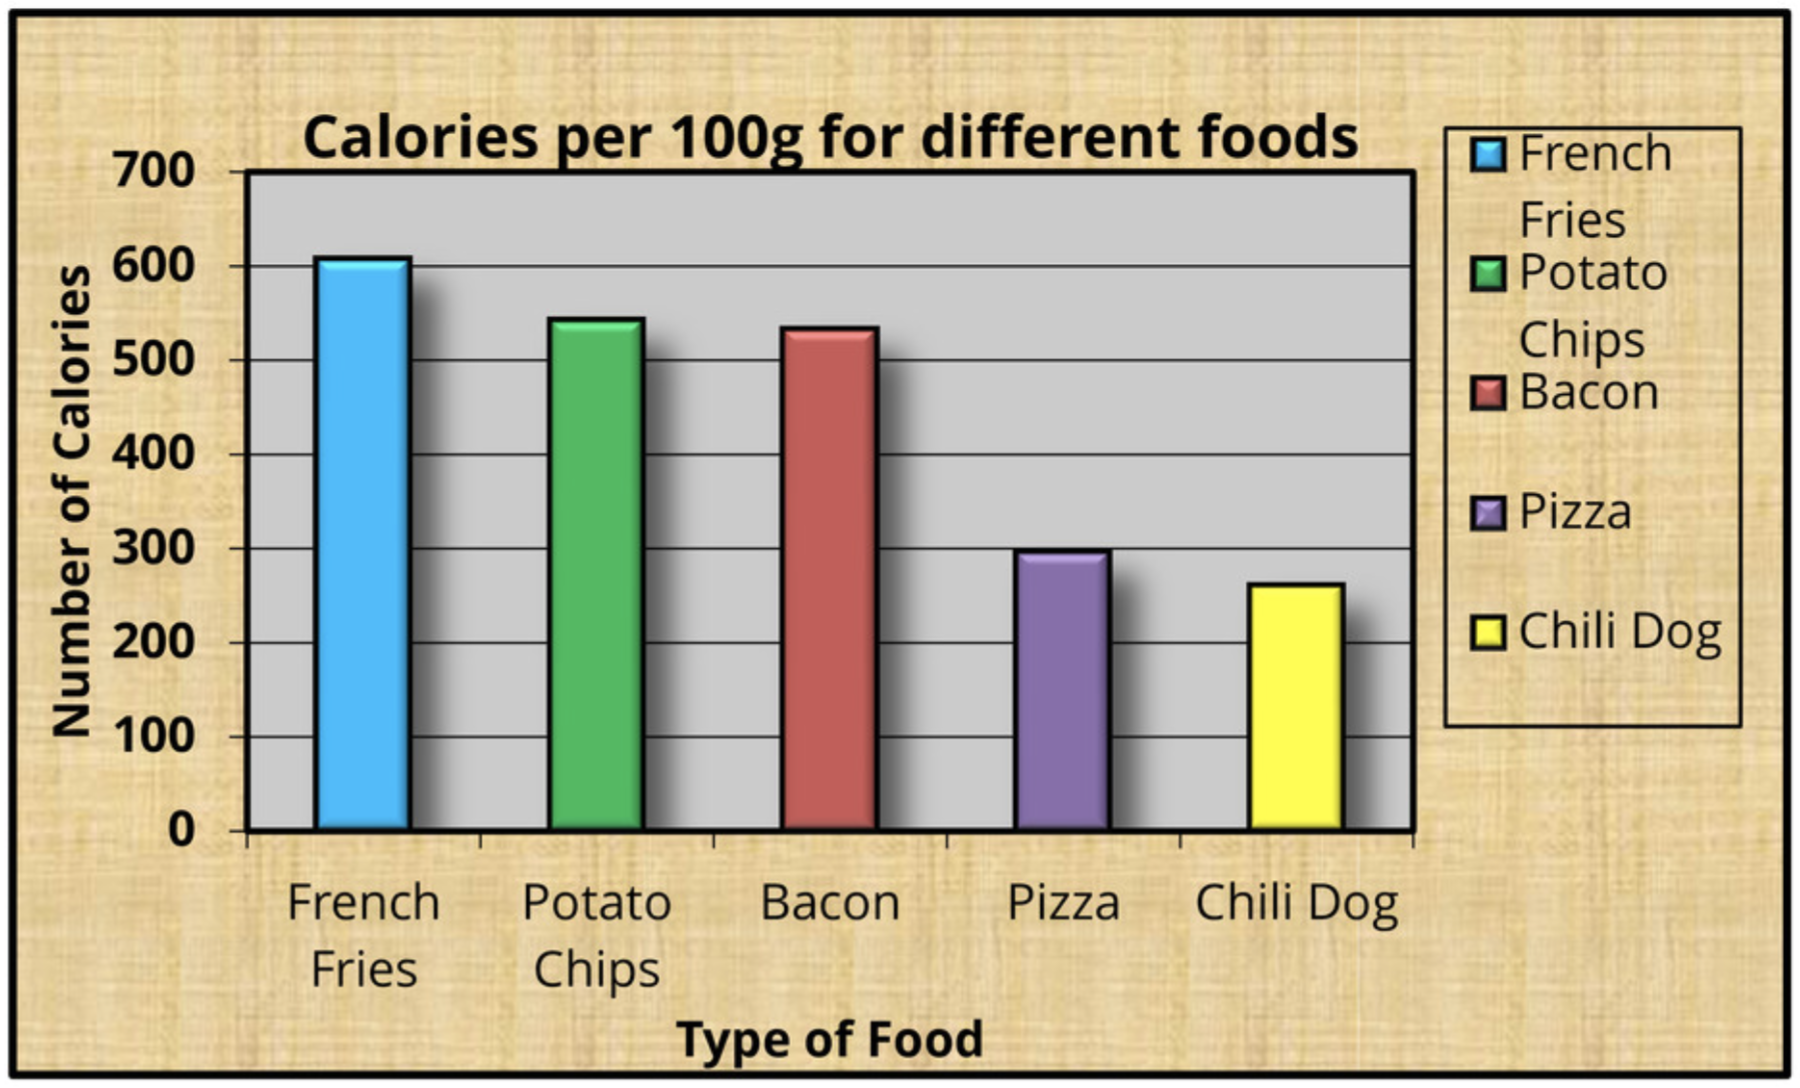
\includegraphics[width=\textwidth]{../figures/barplot-before}
% 	\caption{This is a fancy barplot.}
% 	\label{fig:barplot-before}
% \end{figure}

\newcommand{\image}[5][t]{
	\begin{figure}[#1]
		\centering
		\includegraphics[width=#2]{../figures/#3}
		\caption{#4}
		\label{fig:#5}
	\end{figure}
}

% Custom command to insert two images next to each other with a margin caption
% This command uses 6 required and one optional arguments/parameters with the following meaning:
%
% Optional:
% 1 - Position of the figure (the default position is 't' for top; if no argument is provided, 't' is used
%
% Required:
% 1 - Path to the frist image (inside the figures folder)
% 2 - Path to the second image (inside the figures folder)
% 3 - Caption of the image
% 4 - Label for the image (a universal fig: is prepended)
%
% Required --------------------------------------------------------------------------------------
% Optional -----------------|		  |			    |					|					    |
% 						    V		  V (1)		    V (2)				V (3)				    V (4)
% Example Usage: \twoimages[h]{barplot-before}{barplot-after}{This is a fancy barplot.}{barplot-sidebyside}
%
% The result will be the same as:
%
% \begin{figure}[h]
% 	\centering
% 	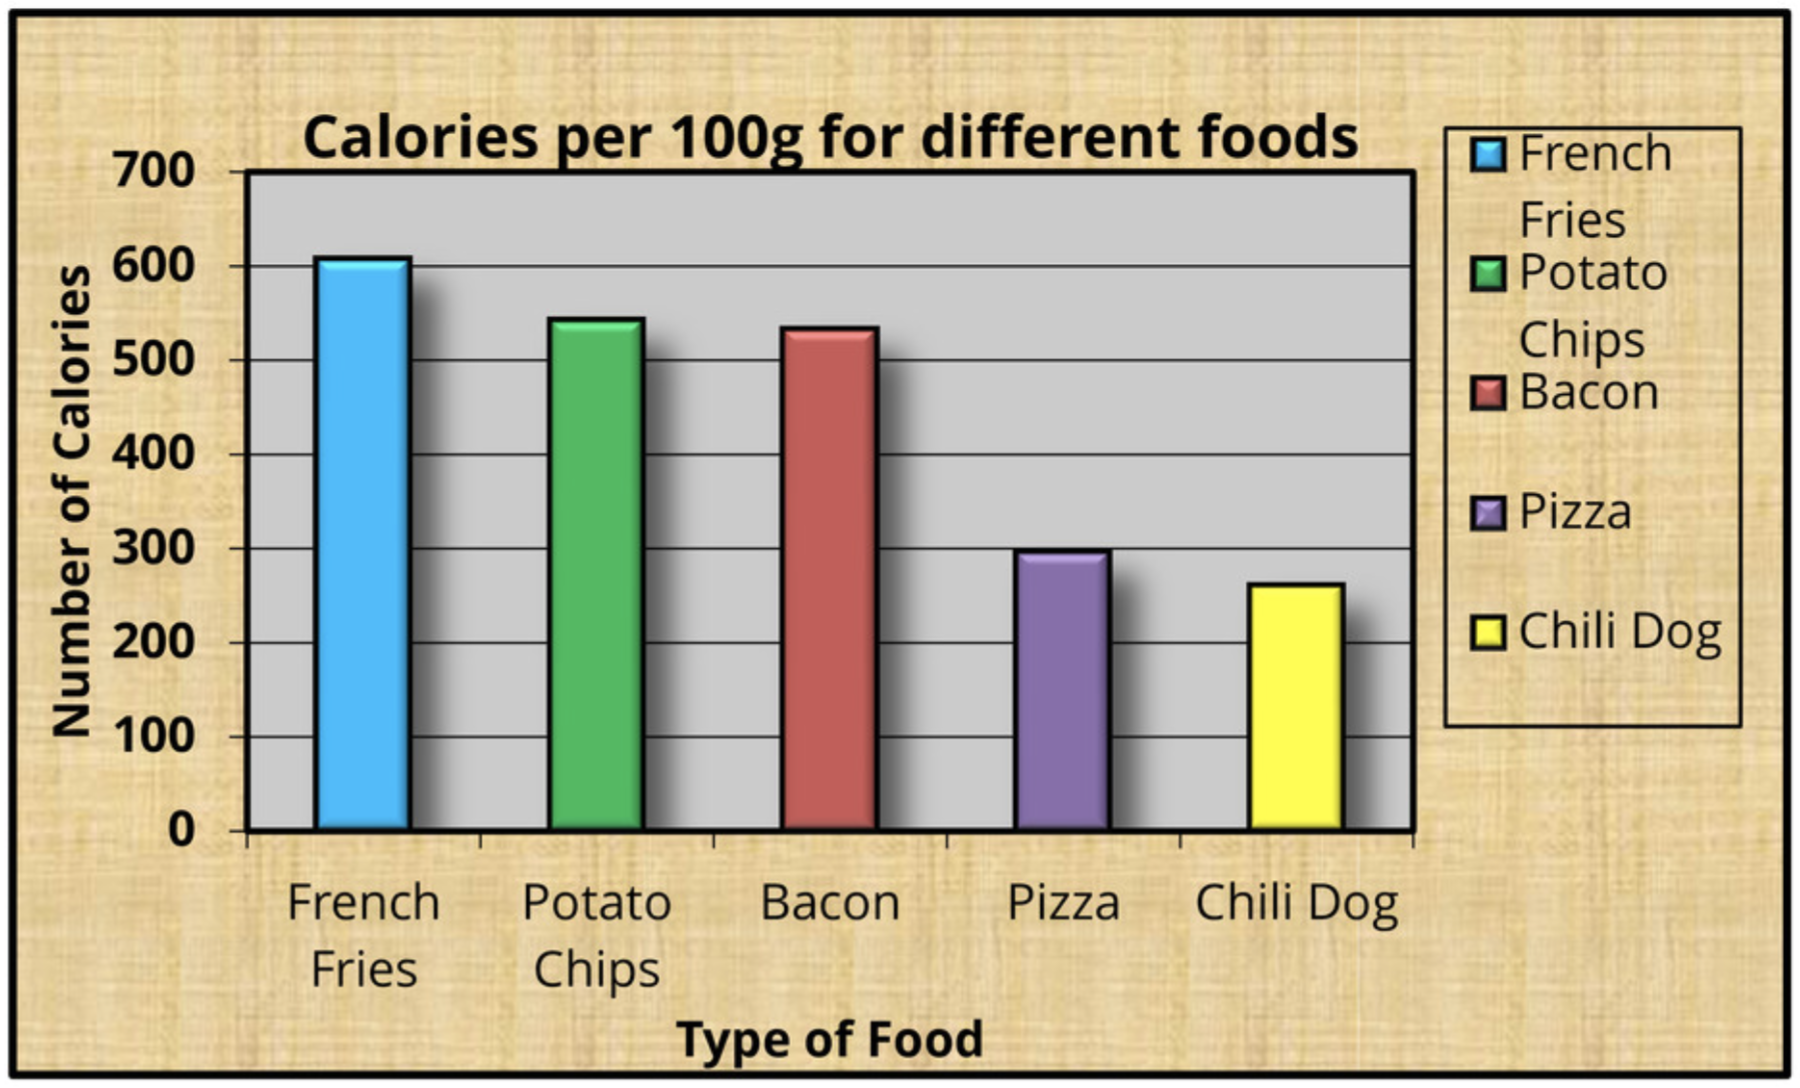
\includegraphics[width=0.48\textwidth]{../figures/barplot-before}
% 	\hspace{\fill}
% 	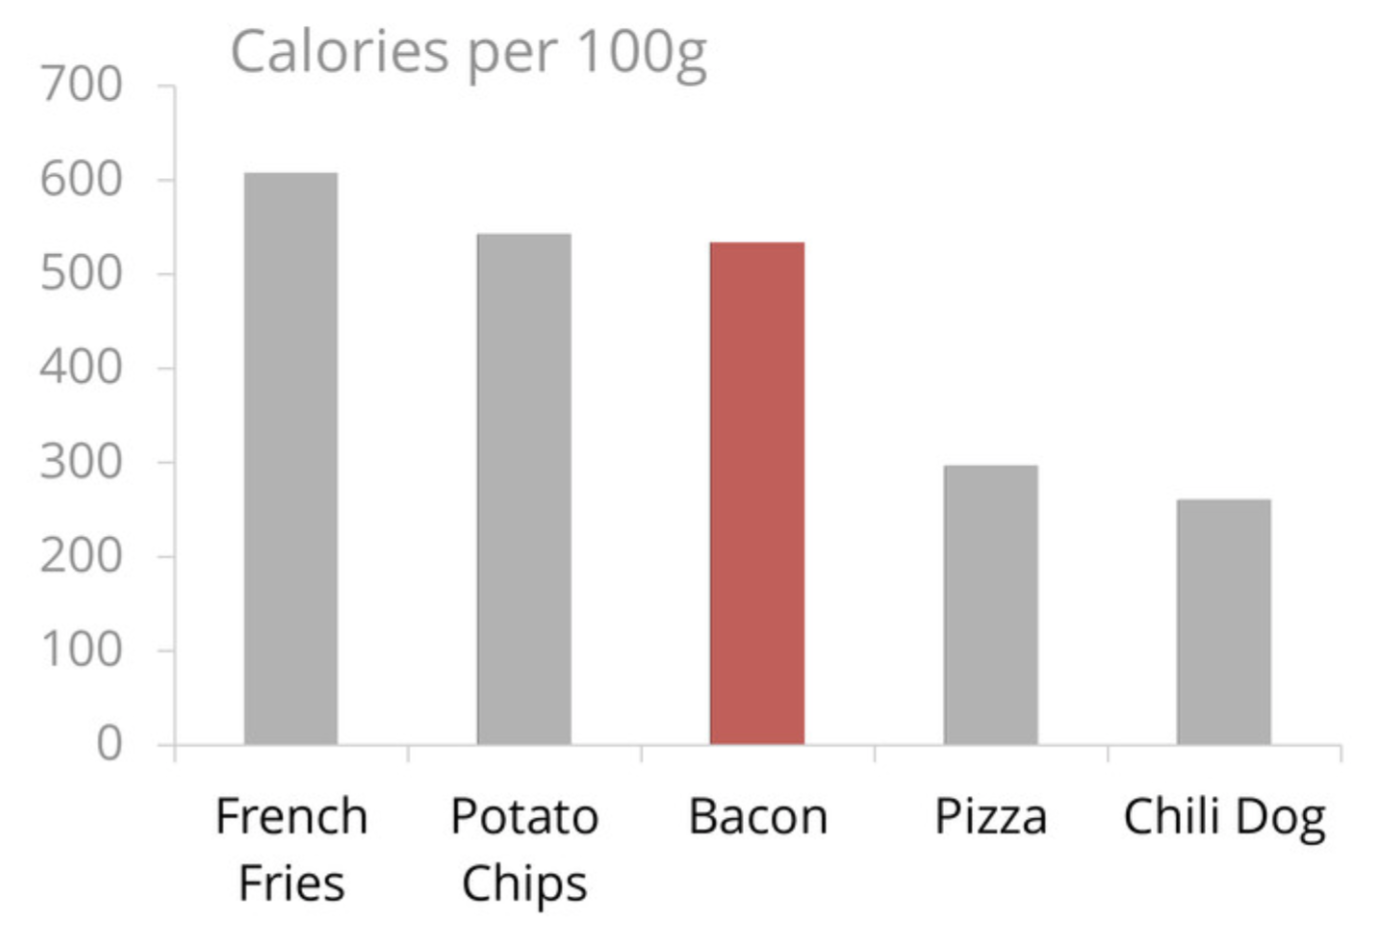
\includegraphics[width=0.48\textwidth]{../figures/barplot-after}
% 	\caption{\label{fig:barplot-sidebyside}This is a fancy barplot.}
% \end{figure}

\newcommand{\twoimages}[5][t]{
	\begin{figure}[#1]
		\centering
		\includegraphics[width=0.48\textwidth]{../figures/#2}
		\hspace{\fill}
		\includegraphics[width=0.48\textwidth]{../figures/#3}
		\sidecaption{\label{fig:#5}#4}[-2\baselineskip]
	\end{figure}
}


% Custom image command for wide figures
% This command uses 4 required and one optional arguments/parameters with the following meaning:
%
% Optional:
% 1 - Position of the figure (the default position is 't' for top; if no argument is provided, 't' is used
%
% Required:
% 1 - Path to the image (inside the figures folder)
% 2 - Caption of the image
% 3 - Label for the image (a universal fig: is prepended)
%
% Required ------------------------------------------------------------------
% Optional -----------------|		  |				 	 |					|
% 						    V		  V (1)		 	  	 V	(2)				V (3)
% Example Usage: \wideimage[h]{barplot-before}{This is a fancy barplot.}{barplot-before}
%
% The result will be the same as:
%
% \begin{figure*}[h]
% 	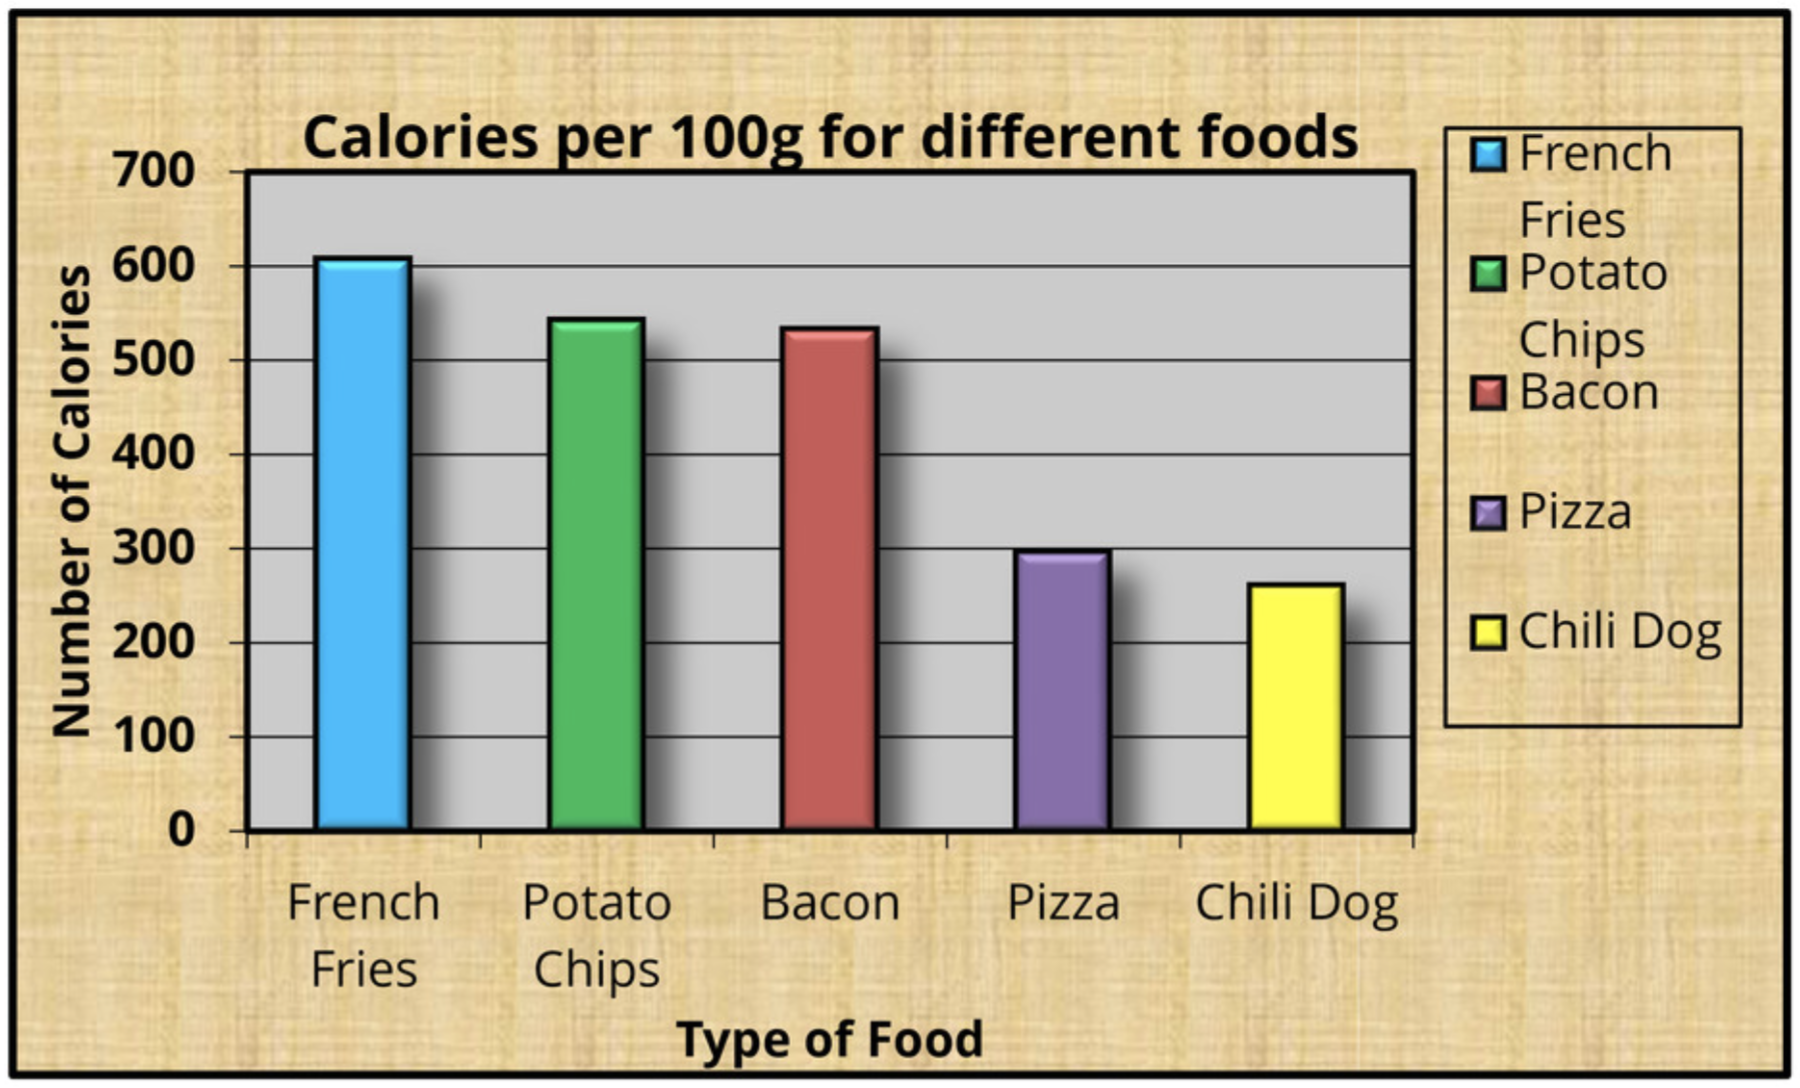
\includegraphics[width=\widefigurewidth]{../figures/barplot-before}
% 	\caption{This is a fancy barplot.}
% 	\label{fig:barplot-before}
% \end{figure*}
%
% %%%%%%%%%%%%%%%%%%%%%%%
% % 	ATTENTION		%
% %%%%%%%%%%%%%%%%%%%%%%%
% It seems this command messes with the position of other images, therefore it is advised to check the placement of other images.

\newcommand{\wideimage}[5][t]{
	\begin{figure*}[#1]
		\includegraphics[width=\widefigurewidth]{../figures/#2}
		\caption{\label{fig:#4}#3}
	\end{figure*}
}

% This command uses 3 required and one optional arguments/parameters with the following meaning:
%
% Optional:
% 1 - Vertical offset of the figure (the default offset is 1 for one line lower (negative numbers move the image up); if no argument is provided, 1 is used
%
% Required:
% 1 - Path to the image (inside the figures folder)
% 2 - Caption of the image
% 3 - Label for the image (a universal fig: is prepended)
%
% Required ----------------------------------------------------------------------
% Optional -------------------|			|				  |						|
% 							  V			V (1)			  V	(2)					V (3)
% Example Usage: \marginimage[2]{barplot-before}{This is a fancy barplot.}{barplot-before}
%
% The result will be the same as:
%
% \begin{marginfigure}[2\baselineskip]
% 	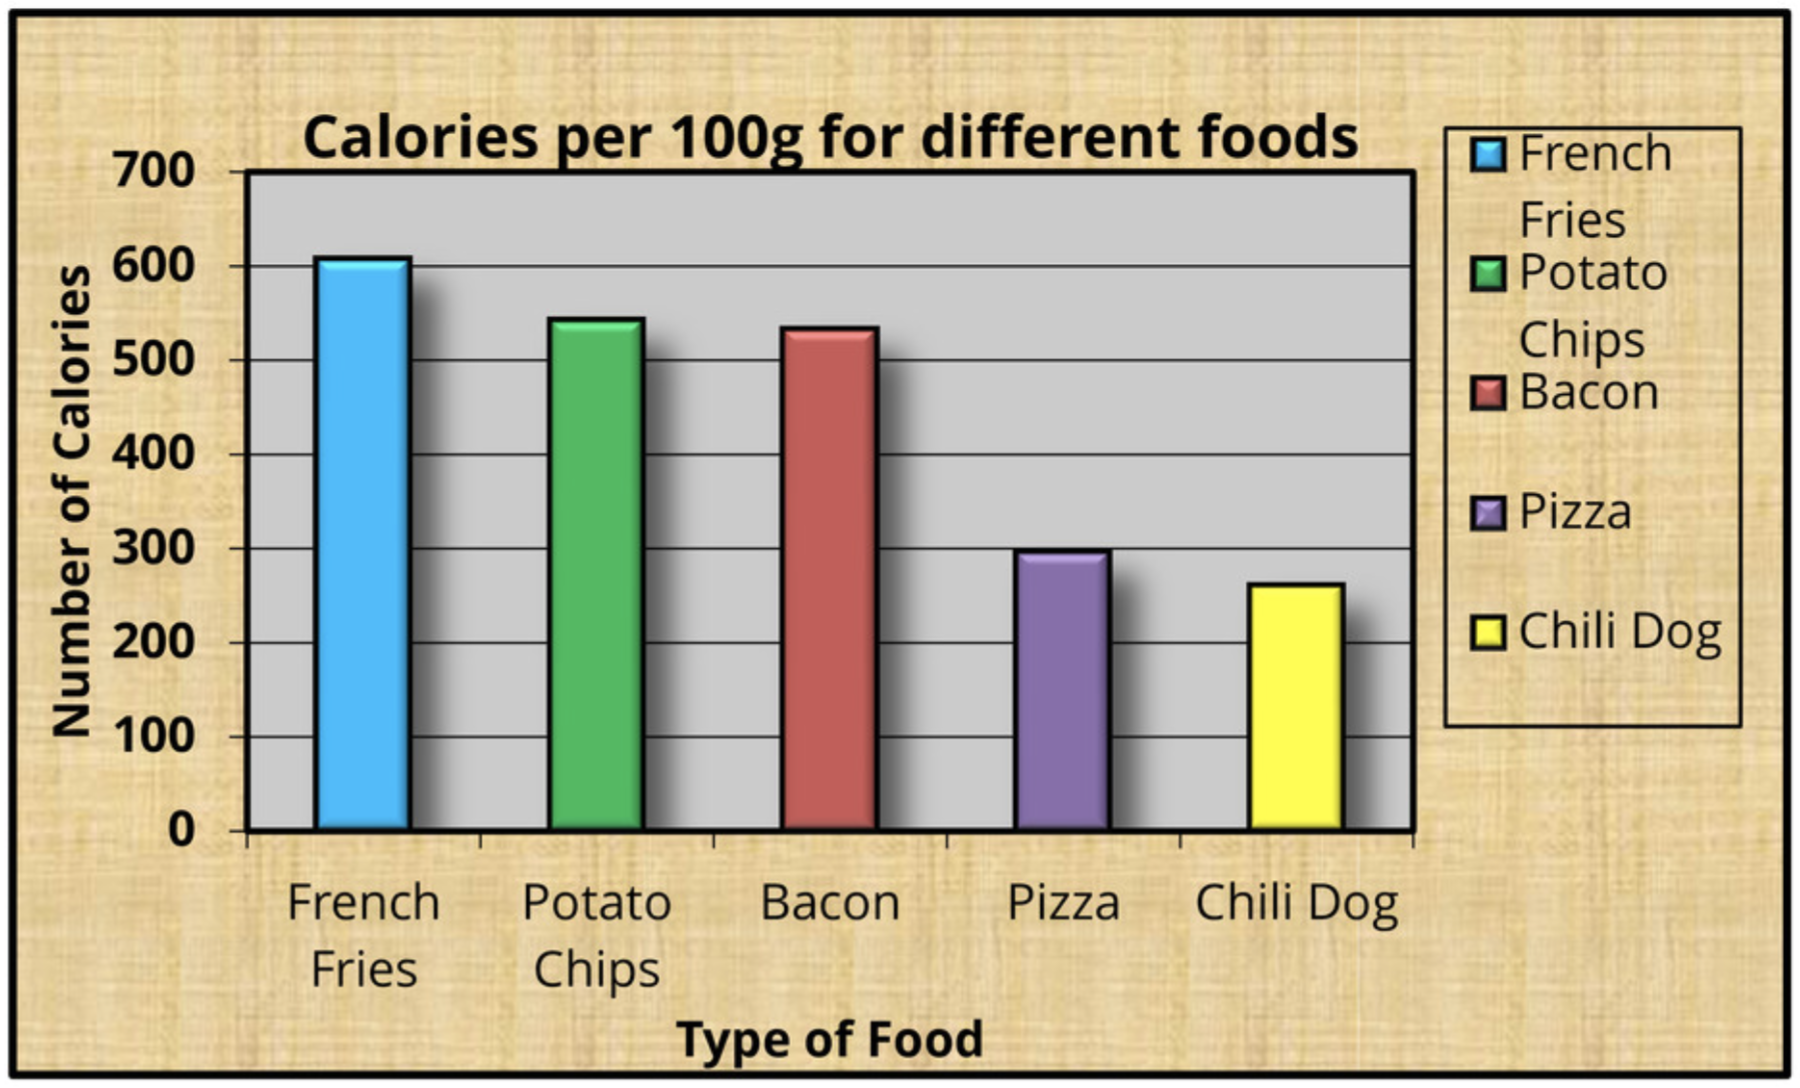
\includegraphics[width=\marginparwidth]{../figures/barplot-before}
% 	\caption{\label{fig:barplot-before}This is a fancy barplot.}
% \end{marginfigure}
\newcommand{\marginimage}[4][1]{
	\begin{marginfigure}[#1\baselineskip]
		\includegraphics[width=\marginparwidth]{../figures/#2}
		\caption{\label{fig:#4}#3}
	\end{marginfigure}
}
 % Load the custom commands from Misc/commands.tex

% Uncomment this command to make all links black:
%   useful for printing on black-white printers that do a
%   poor job at rasterizing colored text properly
%\hypersetup{colorlinks=false}

\addbibresource{literature.bib} % The filename of the bibliography

%----------------------------------------------------------------------------------------
%	THESIS INFORMATION
%----------------------------------------------------------------------------------------
\newcommand{\thesistype}{Master} % type of your thesis (Bachelors, Masters, Doctoral ...)

%%% CHANGE THIS:
% Your thesis title, this is used in the title and abstract, print it elsewhere with \ttitle
\thesistitle{Entwicklung eines interaktiven Werkzeugs zur Kuratierung von Umweltdaten einer bürgerinitiierten Crowdsensing-Kampagne}

% date to be printed on the title, this will automatically update and be in the correct format
% If any changes to this format (Month JJJJ) are necessary the definition can be found in line 337
% of misc/setup.tex
\def\tdate{15.\ November 2023}%\monthyeardate\today}

%%% CHANGE THIS:
% Your name, this is used in the title page, print it elsewhere with \authorname
\author{Samet Murat Akcabay}

% Your supervisor's name, this is used in the title page, print it elsewhere with \supname
\supervisor{Leonie Ackermann \\ Prof.\ Dr.\ Daniela Nicklas}

% Your university's name and URL, this is used in the title page, print it elsewhere with \univname
\university{\href{https://www.uni-bamberg.de/}{Otto-Friedrich-Universität Bamberg}}

% Your research group's name and URL, this is used in the title page, print it elsewhere with \groupname
\group{\href{https://www.uni-bamberg.de/en/mobi/}{Lehrstuhl für Informatik, insbesondere Mobile Softwaresysteme/Mobilität}}

% Your department's name and URL, this is used in the title page, print it elsewhere with \deptname
\department{department not used}

% Your faculty's name and URL, this is used in the title page, print it elsewhere with \facname
% TODO: insert *your* degree program in the \faculty command below
% Applied Computer Science
% Computing in the Humanities
% Information Systems
% International Information Systems Management
% International Software Systems Science
% Software Systems Science
% Education in Business and Information Systems
\faculty{Angewandte Informatik an der \\ \href{https://www.uni-bamberg.de/wiai/}{Faktultät Wirtschaftsinformatik und Angewandte Informatik}}

% Your address, this is not currently used anywhere in the template, print it elsewhere with \addressname
\addresses{address not used}

% Your subject area, this is not currently used anywhere in the template, print it elsewhere with \subjectname
\subject{subject not used}

% Keywords for your thesis, this is not currently used anywhere in the template, print it elsewhere with \keywordnames
\keywords{keywords not used}
%----------------------------------------------------------------------------------------
%	END OF THESIS INFORMATION
%----------------------------------------------------------------------------------------


\begin{document}

\selectlanguage{ngerman}

\frenchspacing % do not add additional hspace after end of sentence full stop dot.

\frontmatter % Uses roman page numbering style (i, ii, iii, iv...) for the pre-content pages

\hypersetup{urlcolor=black}

%%%%%%%%%%%%%%%%%%%%%%%%%%%%%%%%%%%%%%%%%%%%%%%%%%%
%
% File: titlepage.tex
% 
% This file is part of the PSIThesis.cls
% LaTeX documentclass
% 
% The code in this file is made available
% under the following license:
%
% LPPL v1.3c (http://www.latex-project.org/lppl)
%
%%%%%%%%%%%%%%%%%%%%%%%%%%%%%%%%%%%%%%%%%%%%%%%%%%%


\pagestyle{plain} % Default to the plain heading style until the thesis style is called for the body content

%----------------------------------------------------------------------------------------
%	TITLE PAGE
%----------------------------------------------------------------------------------------

\begin{titlepage}

\newgeometry{
	inner=4cm, % Inner margin
	outer=4cm, % Outer margin
	marginparwidth=0cm,
	marginparsep=0mm,
	bindingoffset=.5cm, % Binding offset
	top=2.5cm, % Top margin
	bottom=2.5cm, % Bottom margin
	showframe % Uncomment to show how the type block is set on the page
}

\begin{center}

\vspace*{.06\textheight}

% The logo of University of Bamberg. Do not use the logo without permission.
% Using it on the title page of a thesis is acceptable.
% TODO Add your own logo here. Do yourself and your readers a favor and use
%      a vectorized logo (PDF) instead of a bitmap (PNG, JPEG)

\includegraphics[width=35mm]{misc/UB_Logo_20mm_CMYK.pdf}

\vspace*{.06\textheight}

{\LARGE \textls[130]{\MakeUppercase{\univname}}\par}\vspace{2\baselineskip} % University name

% TODO uncomment the next line when you write a thesis to display the supervisor
%{\large \facname}
% TODO comment out the next line when you write a thesis
{\large ~} % For use in the guide

\vspace{1.5cm}

% TODO uncomment the next line when you write a thesis to display the supervisor
%\textsc{\Large \thesistype 's~Thesis}\\[1cm] % For use in the thesis
% TODO comment out the next line when you write a thesis
\textsc{\Large ~}\\[1cm] % For use in the guide

%\HRule \\[0.4cm] % Horizontal line
%
{\huge \bfseries \ttitle\par}\vspace{1cm} % Thesis title

%\HRule \\[1.5cm] % Horizontal line


\textsc{\Large by}\\[1cm]

{\Large \authorname}

\vspace{1.5cm}

% TODO uncomment the next two lines when you write a thesis to display the supervisor
%\emph{Supervisor:} \\
%\supname\\[1cm]
%% 

\groupname%\\[2cm] % Research group name and department name

\vfill

{\large \tdate} % Date

% TODO remove the following lines when you write a thesis
\vspace{0.25ex}

{\small \tversion}

\vspace{0.25ex}

{\small Links to this document:}\\
{\small \url{\doiurl}} (initial version)\\
{\small \url{\githuburl} (most recent version)}
% Remove lines up to this line

\vfill
\end{center}

\restoregeometry

\end{titlepage}


 % Typeset the titlepage

\hypersetup{urlcolor=ubblue80}


%----------------------------------------------------------------------------------------
%	QUOTATION
%----------------------------------------------------------------------------------------

% \vspace*{0.2\textheight}

% \noindent\enquote{\itshape Thanks to my solid academic training, today I can write hundreds of words on virtually any topic without possessing a shred of information, which is how I got a good job in journalism.}\bigbreak

% \hfill Dave Barry


%----------------------------------------------------------------------------------------
%	ABSTRACT PAGE
%----------------------------------------------------------------------------------------

\begin{abstract}
%\addchaptertocentry{\abstractname}

\end{abstract}


%----------------------------------------------------------------------------------------
%	ACKNOWLEDGEMENTS
%----------------------------------------------------------------------------------------

\begin{acknowledgements}
% %\addchaptertocentry{\acknowledgementname}
% Add the acknowledgements to the table of contents (not recommended)
%
Prof.\ Dr.\ Thomas Foken
Bürgerverein Bamberg Mitte e.V.\
\end{acknowledgements}


%----------------------------------------------------------------------------------------
%	TABLE OF CONTENTS
%----------------------------------------------------------------------------------------

\cleardoublepage
% Table of Contents uses a wider layout than the main content
\newgeometry{
		head=13.6pt,
		top=27.4mm,
		bottom=27.4mm,
		inner=24.8mm,
		outer=24.8mm,
		marginparsep=0mm,
		marginparwidth=0mm,
}
{
\hypersetup{linkcolor=black}
\tableofcontents % Prints the ToC entries
}
\restoregeometry
%----------------------------------------------------------------------------------------
%	DEDICATION
%----------------------------------------------------------------------------------------

% \dedicatory{For/Dedicated to/To my\ldots}


%----------------------------------------------------------------------------------------
%	THESIS CONTENT - CHAPTERS
%----------------------------------------------------------------------------------------
\mainmatter% From here on, numeric (1,2,3...) page numbering
\pagestyle{thesis} % Return the page headers back to the "thesis" style

% Define some commands to keep the formatting separated from the content
\newcommand{\keyword}[1]{\textbf{#1}}
\newcommand{\tabhead}[1]{\textbf{#1}}
\newcommand{\code}[1]{\texttt{#1}}
\newcommand{\file}[1]{\texttt{#1}}
\newcommand{\option}[1]{\texttt{\itshape#1}}

% Figures will automatically be searched for in the Figures subdirectory
\graphicspath{{./figures/}{./examples/}}

%%% CHANGES NEEDED HERE
%
% Include the chapters of the thesis as separate files from the Chapters folder
% Uncomment the lines as you write the chapters
% Mind the \input instead of the \include here, that change is necessary for the appendix formatting
% Due to the \input command you also need to provide the .tex file ending
\addchap{Abkürzungsverzeichnis}
\begin{acronym}
    \acro{acro}[Abkürzung]{Dies ist eine Abkürzung}
\end{acronym}
\chapter{Einleitung} % Kapitel zur Einleitung
\enquote{Die Herausforderungen unserer Zeit sind zu groß, als dass ein Mensch sie alleine lösen könnte} - so lautet ein Auszug der Partei GRÜNE in ihrem Regierungsprogramm\sidenote{\url{https://www.gruene-bayern.de/programm/}} für die Landtagswahl 2023 in Bayern. Mit diesem Slogan bezieht sich die Partei darauf, politische Ziele in Form vom Bau bezahlbarer Wohnungen in Gemeinden, der Planung von Windrädern mit Nachbarorten zu verwirklichen, und das alles auf eine sichere und klimaneutrale Lebensweise. \\ Diese Denkweise kann immer häufiger in der Gesellschaft beobachtet werden, wenn große Unternehmen wie Apple, BMW und IBM, obwohl sie aus unterschiedlichen Domänen stammen, mit demselben Ziel an die Öffentlichkeit treten: der Nachhaltigkeit. Elektronische Geräte wie Smartphones und Notebooks werden mit 100\% recycelten Materialien\sidenote{\url{https://www.apple.com/de/iphone-15-pro/}} hergestellt, während Automobilhersteller auf vollelektrische Automodelle unter der Einhaltung der Klimaneutralität\sidenote{\url{https://www.bmw.de/de/topics/service-zubehoer/bmw-special-sales/sustainability/bmw-special-sales-sustainability-hub-uebersicht.html}} setzen. Die Motivation hinter diesem Umdenken ist der Klimawandel, denn die CO2-Emissionen auf der Welt haben sich seit 1960 von knapp 10.000 Tonnen CO2eq\sidenote{Formelzeichen für das Treibhauspotenzial} auf knapp 40.000 Tonnen CO2eq bis 2021 vervierfacht \cite{GlobalCarbonAtlas2023}. Als Industrieland trägt Deutschland maßgeblich zum Ausstoß der Treibhausgase bei, denn hier kommen weiterhin 53,7\% konventionelle Energieträger\sidenote{Kohle, Kernenergie und Erdgas} im industriellen, aber auch privaten Sektor zum Einsatz \cite{StatistischesBundesamt2023}. Mit dieser Bilanz hat Deutschland 2021 den siebthöchsten Ausstoß an CO2-Emissionen mit 674,75 Tonnen CO2eq im weltweiten Vergleich \cite{GlobalCarbonAtlas2023}. \\
Umso wichtiger ist es also, den Aspekt der Nachhaltigkeit im Zuge des Klimawandels in immer mehr Bereiche des Alltags zu integrieren. Einer dieser Bereiche ist die Softwareentwicklung, denn Software ist in der heutigen Zeit in allen Bereichen des Lebens zu finden, unabhängig davon, ob im privaten Sektor, in der Industrie oder in der Politik. Aufgrund dessen ist es wichtig, dass Softwareentwickler*innen sich mit dem Thema der Nachhaltigkeit auseinandersetzen und Lösungen entwickeln, die diesen Aspekt berücksichtigen.

Motiviert durch die Nachhaltigkeit und den Klimawandel, wird in Bamberg seit Anfang 2022 auf Initiative des \ac{BVM} ein Klimamessnetz\sidenote{\url{https://bvm-bamberg.de/de/projektseiten/klima/}} betrieben, welches die Temperatur und die Luftfeuchtigkeit an verschiedenen Standorten innerhalb der Stadt misst. Die Messungen erfolgen dabei durch smarte Wetterstationen von Netatmo\sidenote{\url{https://www.netatmo.com/de-de/smart-weather-station}} und die Auslesungen können auf einer interaktiven Karte in einer für diesen Einsatz vorgesehenen Webapplikationen\sidenote{\url{https://weathermap.netatmo.com/}} in Echtzeit ausgelesen werden. Das Ziel des Klimamessnetzes ist es, ein grundlegendes Verständnis über das Klima in Bamberg zu erhalten, um Verantwortungspersonen, wie Politiker*innen, Stadtplaner*innen und Ämter, zu erreichen und die Stadt nachhaltiger zu gestalten. \\ Ein Rückschritt beim Erreichen dieses Ziels sind auftretende Fehler und Anomalien in den Auslesungen der smarten Wetterstationen: Durch exogene Einflüsse\sidenote{z.B. Stationen werden verdeckt oder durch reflektierende Fenster direkt von der Sonne angestrahlt, Wärmestrahler von Gaststätten und Restaurants werden in unmittelbarer Nähe eingeschaltet oder Vergleichbares} auf die Stationen treten Ausreißer in den Auslesungen auf, die die Sensordaten, und damit die Repräsentativität der Daten negativ beeinflussen. 

Diese Arbeit soll gleichzeitig eine Lösung für das beschriebene Problem des Klimamessnetzes in Bamberg und einen Beitrag durch die Bereitstellung einer Softwarelösung motiviert durch den Klimawandel bieten. Dabei wird das Klimamessnetz aufgegriffen und durch den Ansatz des Crowdsensings erweitert. Konkret bedeutet dies, dass Bürger*innen der Stadt Bamberg durch den Einsatz eines interaktiven Werkzeugs in der Lage sein sollen, die Umweltdaten insofern zu kuratieren\sidenote{Mit der Kuratierung wird in dieser Arbeit die Tätigkeit bezeichnet, erfasste Daten auf ihren repräsentativen Wert zu bewerten und darauf basierend zu kategorisieren (\textit{lateinisch:} \enquote{sich kümmern um})}, sodass auftretende Ausreißer, Anomalien und Fehler in den Sensordaten auf ein Minimum begrenzt werden können. Mit diesem Prozess wird außerdem präsentiert, wie die Vorgehensweise der Softwareentwicklung durch den Crowdsensing-Ansatz beeinflusst wird. Im Anschluss wird die Softwarelösung als Artefakt genutzt, um die aus dem Crowdsensing-Ansatz resultierenden Vor- und Nachteile auf die Software selbst, aber auch den Einsatz dieser zu evaluieren. Konkret soll die folgende Forschungsfrage beantwortet werden: 

\textbf{Wie plant und entwickelt man eine Softwarelösung zur Kuratierung von Umweltdaten einer bürgerinitiierten Crowdsensing-Kampagne?} 


Um diese Frage zu beantworten, ist die Arbeit wie folgt strukturiert: Zunächst wird der Hintergrund dieser Arbeit präsentiert, um eine Grundlage für die nachfolgenden Kapitel zu schaffen. Auf dieser Grundlage basiert das Konzept, welches die Softwarelösung konzeptuell beschreibt, die im Anschluss in der Implementierung umgesetzt wird. Vor der Implementierung ist es aber erforderlich, die Anforderungen an die Software zu definieren, um die Umsetzung zu erleichtern. Nach der Implementierung wird die Software evaluiert, um die Vor- und Nachteile des Crowdsensing-Ansatzes in der Softwareentwicklung zu präsentieren, aber auch den gesamten Prozess dieser Arbeit zu bewerten. Aus dieser wird ein Fazit gezogen, welches die Frage beantwortet, ob der Crowdsensing-Ansatz in der Softwareentwicklung sinnvoll ist und in zukünftigen Implementierungen berücksichtigt werden soll.
\chapter{Hintergrund} % Kapitel zum theoretischen Hintergrund
%%muss halt dargestellt sein, warum ich was gemacht hab (verwandte arbeiten) Hintergrund ist dafür da, ich hab das thema recherchiert, kenn mich damit aus aber soll auch zeigen "inwiefern kenn ich mich damit aus?"
In diesem Abschnitt der Arbeit geht es darum, eine Grundlinie des theoretischen Hintergrunds zu schaffen. Dieser Aspekt wird dadurch umgesetzt, indem zunächst der Begriff des \enquote{Crowdsensings} mit dem in der Literatur weitverbreiteten Begriff des \enquote{Crowdsourcings} abgegrenzt wird. Infolgedessen ist es somit in den folgenden Kapiteln möglich, den Begriff des Crowdsensings in den Kontext der Arbeit zu setzen. Im Anschluss werden verwandte Arbeiten vorgestellt, welche sich mit dem Thema des Crowdsensings und der Umsetzung von Plattformen mit diesem 
Hintergrund beschäftigen.

\section{Crowdsensing vs. Crowdsourcing}
% Hier mit Verwandten Arbeiten vergleichen
In der Literatur wird der Begriff des (mobilen) Crowdsensings durch das Vorhandensein einer großen Anzahl an Teilnehmenden für eine großflächige Überwachung der Umwelt beschrieben, welche rohe Daten mithilfe von in smarte Geräte eingebettete Sensoren messen \cite{Ray2022}. Um an den Begriff des Crowdsensings heranzutreten, wird aber zunächst zwischen zwei Arten des Messens unterschieden: dem sogenannten \enquote{personal sensing}, in dessen Anwendung Individuen persönliche Informationen aus eigenem Interesse oder Bedarf (z.B. Messungen zum Überwachen der eigenen Gesundheit, aber auch zum Nachverfolgen von persönlichen Rekorden oder dem ökologischen Fußabdruck) messen und dem \enquote{community sensing}, bei welchem großflächige Phänomene, welche durch einzelne Individuen nicht gemessen werden können, untersucht werden \cite{Ganti2011}. \newline Als Beispiele können hierfür sämtliche Anwendungsfälle genannt werden, in denen die Teilnahme von mehreren Individuen (unter Umständen zur selben Zeit) unabdingbar ist, wie beim Messen der Temperatur, der Luftfeuchtigkeit oder der Luftqualität an verschiedenen Orten. Der Begriff des \enquote{community sensing} kann hierbei weiterhin in zwei Kategorien unterteilt werden, dem sogenannten \enquote{participatory sensing} \cite{Burke2006} und dem \enquote{opportunistic sensing} \cite{Lane2010}: \newline Während bei Ersterem eine aktive Teilnahme, verbunden mit eigenmotiviertem Aufwand (z.B. Aufnahme von Fotos, Eingabe und Übermittlung von Information), notwendig ist, wird bei Letzterem eher ein minimaler Aufwand durch eine selbstständige Messung der Sensoren (z.B. kontinuierliche Temperaturmessung der Sensoren in Abhängigkeit vom Standort, ohne Eingaben der Nutzenden) betrieben \cite{Ganti2011}. Aus diesem Grund bildet der Begriff des Crowdsensing in der Literatur keine eindeutige Art der Messung, sondern vielmehr eine Domäne der genannten Arten an Messungen durch eine Gruppe von Individuen \cite{Ganti2011}. \newline Das mobile Crowdsensing kann in drei Schritte unterteilt werden: der Datenerhebung, der Datensammlung und dem Datenupload \cite{Ray2022}. Die Datenerhebung erfolgt sowohl durch die User, als auch durch \enquote{mobile sensing devices} (z.B. Thermometer, Smartphones etc.), welche auf einem Server gesammelt werden um im Anschluss hochgeladen werden können, um sich z.B. einer Qualitätskontrolle zu unterziehen \cite{Ray2022}. Die Vorteile des mobilen Crowdsensing erstrecken sich dabei von schneller Erhebung von vielfältigeren Daten mit erhöhter Qualität der Ergebnisse, bis hin zu akzeptableren Ergebnissen und das Auslagern von Rechenleistung von einer zentralen Plattform zu bspw. den mobilen Geräten \cite{Ray2022}. Auf der anderen Seite kann man jedoch beobachten, dass die erhobenen Daten geprägt von Redundanzen und Duplikaten sind, was zur Folge hat, dass eine 
anschließende Qualitätskontrolle und die Notwendigkeit von mehr Speicherplatz unabdingbar sind \cite{Ray2022}. Es lassen sich häufig Smartphones als Messgeräte des mobilen Crowdsensing in der Literatur finden, da diese mit einer vielzahl an Sensoren (Temperatur-, Gyroskop-, Umgebungslichtsensoren etc.) ausgestattet sind - das mobile Crowdsensing ist aber nicht auf diese limitiert und beinhaltet auch Geräte wie mobile Wetterstationen, Bewegungssensoren, Kameras o.Ä. 

Das mobile Crowdsourcing ermöglicht das Lösen einer komplexen Aufgabe durch die Auf- und Verteilung von Aufgaben an eine Gruppe von freiwilligen Nutzenden, hier über das Internet \cite {Wang2019}. Die Komposition \enquote{Crowdsourcing} besteht dabei aus den beiden einzelnen Begriffen \textit{crowd} für die (Menschen-)Menge und \textit{sourcing} für die Beschaffung (hier: von Informationen). Erstmalig wurde der Begriff 2006 vom Journalisten Jeff Howe in einem Artikel verwendet, welcher das Crowdsourcing als kostengünstigere Alternative des \textit{Outsourcing}\sidenote{zu deutsch: Auslagerung, \enquote{mittel- bis langfristige Übertragung von Aufgaben der Informationsverarbeitung eines Unternehmens an ein spezialisiertes Unternehmen} \cite{Heinrich2014}} beschreibt, um Akteure aus unterschiedlichen Wissensständen und Domänen in die Softwareentwicklung miteinzubinden \cite{Howe2006}. Im weiteren Verlauf der Verwendung des Begriffs spielen die Charakteristiken ebenfalls eine Rolle: Die Lösung eines Problems wird insofern erreicht, dass die Aufgaben (und unter Umständen auch Unteraufgaben, abhängig von Problemstellung) an eine (Menschen-)Menge übertragen werden, welche interessiert an der Lösung des Problems sind \cite{Ray2022}. Weiterhin wird die Verteilung der Menge 
und die Existenz von variierender Menschenlogik genutzt, um Probleme an jenen Computer scheitern, zu lösen \cite{Ray2022}. Der Unterschied zum Crowdsensing ist hierbei, dass die verrichtete Arbeit nicht auf die Interaktion mit Geräten und den entsprechenden Sensoren ist, sondern dass Arbeit im Allgemeinen verrichtet wird (vergleiche Parallele zwischen Crowdsourcing und Outsourcing). Beim Einsatz vom mobilen Crowdsensing ist vorteilhaft, dass Kosten durch nicht-benötigte Arbeitskräfte basierend auf einer expliziten Arbeitszeit verringert sind, der Einsatz einer Menge als Folge davon eine vielfältigere und qualitativ hochwertigere Datensammlung nach sich zieht und die Verfügbarkeit von vielfältigen Parametern zum Testen in Summe in eine hohe Zeitersparnis resultieren \cite{Ray2022}.

Aus den Definitionen der beiden Begriffe wird deutlich, dass diese viele Gemeinsamkeiten aufweisen, was der Grund dafür ist, dass in der Umgangssprache, aber auch in der Literatur eine Verwechslung beider Begriffe auftreten kann. Aufgrund dessen ist es erforderlich, die Abgrenzung der Begriffe voneinander hervorzuheben, welche sich in der Bearbeitung der Aufgaben und der Notwendigkeit von menschlicher Intelligenz findet: Während das mobile Crowdsensing die Aufgaben auf das Erfassen von Rohdaten begrenzt, erstrecken sich Aufgaben beim Crowdsourcing über die Erfassung von Rohdaten bis zu anderen, von der Plattform zugewiesenen (allgemeinen) Aufgaben hinaus \cite{Ray2022}. Für eben diese Aufgaben wird dementsprechend auch eine bestimmte menschliche Intelligenz vorausgesetzt, die mit der Rechenleistung zusammenarbeiten soll, um eine Lösung zu finden \cite{Ray2022}.

\section{Verwandte Arbeiten}
% Hier mit Verwandten Arbeiten vergleichen
Der Aspekt des Crowdsensing lässt sich sowohl in der Literatur, als auch in der Praxis durch bereits existierende Projekte und Anwendungen vorfinden. Um ein grundlegendes Verständnis über das Thema und zur Definition eines theoretischen Rahmens zu schaffen, wurden diese verwandten Arbeiten herangezogen, welche in diesem Kapitel vorgestellt werden. \newline Bei der ersten Arbeit handelt es sich um \enquote{Crowdsensing für Bodensee Online}, ein von der ISB AG, vom Fraunhofer-Institut für Optronik, Systemtechnik und Bildauswertung und der Ingenieurgesellschaft Prof. Kobus und Partner GmbH im Februar 2020 initiiertes Projekt zur Messung der Wassertemperatur des Bodensees durch Bootsbesitzer*innen mithilfe von mobilen Sensoren und Karten \cite {Ministerium2021}. Der Fokus des Projekts liegt darin, die bereits vorhandenen Kenntnisse über die Verhältnisse am Bodensee durch einen citizen-science Ansatz zu erweitern und auf die Durchführbarkeit zu messen \cite{Bodensee2021}. Dabei sollte zunächst in einer Pilotphase die Funktionsweise und die Montagemöglichkeit der Sensoren vor Ort erprobt werden, um im Anschluss mit ausgereiften Sensoren in die Feldphase zu starten, in welcher die Probanden mithilfe der Sensoren mit den Messungen des Bodensees beginnen konnten \cite{Bodensee2021}. Aufgrund der COVID-19 Pandemie und den damit vorherrschenden Einschränkungen verliefen beide Phasen überlappend zueinander, sodass eine kontinuierliche Weiterentwicklung der Sensoren und der Nutzeroberfläche basierend auf den Erfahrungen der Nutzenden möglich gewesen wäre \cite{Bodensee2021}. Im Allgemeinen beschreiben die Durchführenden des Projekts die Ergebnisse als sehr positiv. \newline In Bezug auf die technischen Aspekte soll der Betrieb, aber auch die Verfügbarkeit der Sensoren keinen Aufwand dargestellt haben. Auch die zuvor aufgestellten Anforderungen seien im breiten Maße erfüllt worden. Lediglich der Aufwand der Standortsuche der Sensoren und die damit verbundene Auswirkung auf die Batterielaufzeit haben eine wesentliche Limitierung dargestellt - eine erste Lösung sei aber dadurch umzusetzen, dass die Sensoren als stationäre Messpunkte einzusetzen wären, um sowohl auf der einen Seite die Messdaten am Bodensee zu erhöhen, aber auf der anderen Seite die Abtastrate des Standortes zu minimieren, um die bereits erwähnten Limitierungen aufzuheben, sodass diese eine plausible Ergänzung zu den stationären Messstationen am Bodensee darstellen \cite{Bodensee2021}. Der Crowdsensing-Ansatz des Projekts wird als geeignet für die Verbesserung und Verfeinerung einer bestehenden (Daten-)Struktur angesehen, da unter der Voraussetzung einer ausreichenden Qualitätssicherung und Datenmenge eine hohe Datenqualität und -dichte auf engem Raum erzielt werden kann \cite{Bodensee2021}. Prinzipiell ließe sich das Projekt laut Angaben der Durchführenden auf weitere (Naturschutz-)Regionen unter Zuhilfenahme weiterer Parameter (z.B. Lufttemperatur, -feuchtigkeit, -qualität) übertragen \cite{Bodensee2021}. Die zugrundeliegenden Charakteristiken schließen darauf, dass es sich bei \enquote{Crowdsensing für Bodensee Online} um \enquote{opportunistic sensing} handelt, da die Sensoren lediglich an die Boote angebracht werden müssen und keine aktive Teilnahme der Bootsbesitzer*innen notwendig ist. 

Aber auch in anderen Domänen ist das Crowdsensing schon zum Einsatz gekommen: Das Projekt \enquote{Track Your Tinnitus}\sidenote{https://www.trackyourtinnitus.org/de/} wurde von der Tinnitus Research Initiative (TRI) und dem Institut für Datenbanken und Informationssysteme (DBIS) der Universität Ulm für medizinische Einsatzzwecke ins Leben gerufen \cite{Pryss2017}. Etwa 10-15\% der Weltbevölkerung leidet unter Tinnitus, einer Krankheit, die durch ein ständiges Ohrgeräusch gekennzeichnet ist und welche bis heute schwer behandelbar ist, da verfügbare Behandlungen nur bei einem Teil der Betroffenen anschlagen \cite{langguth2011review}. Da klinische Tests und Versuche bisher den Standard repräsentiert haben, und die damit verbundene Informationsgewinnung sehr begrenzt gewesen ist, wurde das Projekt ins Leben gerufen, um eine komplementäre Vorgehensweise vorzuschlagen, die durch den Einsatz von Crowdsensing-Services die Datenerhebung vereinfacht, aber auch vervielfacht \cite{pryss2015mobile}. Die Nutzenden sollen dabei eine Smartphone-App installieren und nach jedem Wahrnehmen des Tinnitus Fragen zur Intensität und Belastung und daraus resultierend, die Auswirkungen auf die persönliche Stimmungslage beantworten, damit individuelle Schwankungen der Tinnituswahrnehmung erfasst werden können \cite{pryss2015mobile}. Einerseits soll es auf diese Weise ermöglicht werden, die behandelnden ärztlichen Fachpersonen mit den notwendigen Daten zu versorgen, um die Behandlung zu verbessern, aber auch das allgemeine Forschungsprojekt zu unterstützen und ein Verständnis für Ursachen und Wirkungen für den Tinnitus zu schaffen \cite{pryss2015mobile}. Die Voraussetzung der Eingabe der persönlichen Tinnituswahrnehmung charakterisiert das Projekt \enquote{Track Your Tinnitus} als \enquote{participatory sensing}, da die Nutzenden aktiv an der Datenerhebung beteiligt sind.

Eine weitere Verwandschaft lässt sich der App \enquote{Budburst}\sidenote{https://budburst.org} zuordnen, welche Nutzende dazu animiert, mithilfe des eigenen Mobiltelefons Pflanzenarten zu identifizieren und in einer Gemeinschaft lokale Pflanzen(-arten) kontinuierlich zu erfassen. Die Nutzenden werden durch die kontinuierliche Erfassung der Pflanzen dazu animiert, den Zustand des lokalen Ökosystems zu überwachen um eventuelle Rückschlüsse auf den Klimawandel ziehen zu können. Durch das Fotografieren von Pflanzen innerhalb der App soll ein Diskurs über die Gesundheit des Ökosystems angeregt werden, welcher durch die Nutzenden und die daraus geformte Gemeinschaft geführt wird. Die App \enquote{Budburst} ist ein Beispiel für \enquote{participatory sensing}, da die Nutzenden ebenfalls aktiv an der Datenerhebung beteiligt sind.

Ausgehend von den genannten Arbeiten und Projekten ist es möglich, weitere verwandte Quellen zu finden, welche sich mit dem Thema des Crowdsensings beschäftigen. Die genannten Arbeiten haben dabei gezeigt, dass das Crowdsensing in unterschiedlichen Domänen zum Einsatz kommen kann, um Problemstellungen zu lösen, welche durch traditionelle Methoden nicht oder nur schwer zu lösen sind.
\chapter{Konzept} % Kapitel zum Konzept
% Grundgedanke hinter dem Tool erläutern, 
% einen Entwurf darstellen und mithilfe von Use Cases verstärken
In diesem Abschnitt der Arbeit geht es darum, das grundlegende Konzept hinter der Entwicklung eines interaktiven Werkzeuges zur Kuratierung 
von Umweltdaten aufzubauen und zu erläutern. Dabei ist es zunächst erforderlich, die allgemeine Umsetzung von Crowdsensing in einer solchen Software zu analysieren, um 
darauffolgend Parallelen zu \enquote{Bamberg messen 2.0} auffinden zu können. \newline Im nächsten Schritt ist es dann erforderlich, den Entwurf näher zu untersuchen damit 
die Nachvollziehbarkeit der Methodologie der Entwicklung gewährleistet ist. Im Anschluss können somit Use Cases aufgestellt werden, um Parallelen zu alltäglichen Ereignissen 
schlagen zu können, sodass die Verwendbarkeit eines solchen Werkzeuges greifbarer wird.
\section{Grundgedanke hinter einem Crowdsensing-Tool}

\section{Entwurf}

\section{Use Cases}
\chapter{Anforderungsanalyse}
\label{sec:requirements}
% Wie ist die Ausgangslage (in Bamberg)? Wie werden/wurden die Anforderungen aufgestellt, 
% wer sind die Stakeholder und warum? Dann Anforderungen definieren und priorisieren
Bevor mit der eigentlichen Implementierung begonnen werden kann, ist es notwendig, die Anforderungsanalyse. Der erste Schritt hierzu besteht daraus, die Ausgangslage in Bamberg zu untersuchen, um darauf aufbauend die Stakeholder zu identifizieren, da diese den Ursprung der Anforderungen darstellen. Nachdem das Aufstellen der Anforderungen erfolgreich gewesen ist, können diese priorisiert und auf ihre Validität und ihre Realisierbarkeit analysiert werden. Basierend auf den Anforderungen werden dann User Stories abgeleitet, die die Anforderungen in einer konkreten Situation aus Sicht der Nutzenden beschreiben. Im Anschluss werden Use Cases präsentiert, um die von außen sichtbare Interaktion mit dem System zu beschreiben.

\section{Ausgangslage in Bamberg}
\label{sec:ausgangslage}
Bamberg\sidenote{\url{https://www.stadt.bamberg.de/Unsere-Stadt/Stadtinfo/}} ist eine kreisfreie Stadt in Bayern im Regierungsbezirk Oberfranken mit einer Einwohnerzahl von knapp 80.000 Einwohnern (Stand: Dezember 2022). Die Stadt selbst kann dabei in sogenannte \ac{LCZ}, also Klassifikationen, welche sich durch die logische Aufteilung einer Landschaft ergeben \cite{stewart2011local}, unterteilt werden. Zusammen mit dem Domänenwissen des Meteorologen Prof.\ Dr.\ Thomas Foken (vgl. Kapitel \ref{sec:stakeholder}) hat eine rudimentäre Unterteilung in sechs \ac{LCZ} stattgefunden: Die Innenstadt, die ERBA, Gartenstadt, Bamberg-Ost, der Hain, am Laubanger und das Berggebiet (siehe Abbildung \ref{fig:lcz}). Die Entscheidung über die Grenzen und der Gebiete erfolgt dabei durch die in der Literatur gegebenen Charakteristika, welche zum Definieren von \ac{LCZ} notwendig sind \cite{oke2004initial, stewart2012local}:

\keyword{Innenstadt (2)} -- Die Innenstadt kann als \enquote{Compact midrise} klassifiziert werden. Charakteristisch für diese \ac{LCZ} ist der dichte Mix aus mittelhohen Gebäuden, das Vorhandensein von wenigen bis keinen Bäumen und hauptsächlich asphaltierten Landflächen. Überwiegend lassen sich Stein, Ziegel, Kacheln und Beton als Baumaterialien vorfinden.

\keyword{ERBA (6)} -- Die ERBA kann als \enquote{Open low-rise} klassifiziert werden. In einem solchen befinden sich in der Regel flache Gebäude, die in einer offeneren Struktur angeordnet sind. Die Landflächen sind asphaltiert, weisen aber auch Grünflächen in Form von kleinen Pflanzen oder verstreuten Bäumen auf. Die Baumaterialien sind ähnlich wie in der Innenstadt, jedoch kann man an der ERBA häufig Holz als Baumaterial vorfinden.

\keyword{Gartenstadt (6B)} -- Die Gartenstadt ist wie die ERBA ein \enquote{Open low-rise}. Allerdings kann hier der Zusatz \textit{\enquote{B}} als \enquote{Land cover type}\sidenote{Nach \cite{stewart2012local}: Klassifikationen zu saisonalen Eigenschaften, wie z.B. schneebedeckter Boden, trockener/feuchter Boden etc.} zur Klassifikation hinzugefügt werden, welche nach \cite{stewart2012local} bedeutet, dass die Landschaft rege mit immergrünen Bäumen bestückt ist. Die Landflächen weisen zu einem Großteil Grünflächen mit kleinen Pflanzen auf. Diese Arten von \ac{LCZ} werden in der Regel für Wälder oder Stadtparks verwendet.

\keyword{Bamberg-Ost (3)} -- Der Osten Bambergs wird als \enquote{Compact low-rise} klassifiziert. Dieser weist die identischen Charakteristika wie die Bamberger Innenstadt auf, mit dem einzigen Unterschied, dass es sich bei den Gebäuden um niedrige Gebäude handelt.

\keyword{Hain (5)} -- Der Hain befindet sich in der Klasse des \enquote{Open midrise}. Dieser weist die identischen Charakteristika wie die ERBA auf, mit dem einzigen Unterschied, dass es sich bei den Gebäuden um mittelhohe Gebäude handelt und statt Holz überwiegend Beton und Stahl als Baumaterialien eingesetzt werden.

\keyword{Laubanger (8)} -- Der Laubanger wird in Bamberg als \enquote{Large low-rise} eingestuft. In dieser Klasse lassen sich in der Regel große, aber flache Gebäude in einer offeneren Struktur vorfinden. Bäume oder Grünflächen sind meistens nicht bis kaum vorhanden, da die Straßen und Wege überwiegend asphaltiert sind. Als Baumaterialien kommen häufig Stahl, Beton und Stein zum Einsatz.

\keyword{Berggebiet (6A)} -- Das Bamberger Berggebiet ähnlich wie die Gartenstadt und ERBA als \enquote{Open low-rise} eingestuft und weist die identischen Charakteristika auf. Der Zusatz \textit{\enquote{A}} besagt hierbei, dass eine große bzw. dichte Menge an Bäumen in der Landschaft vorzufinden ist, was in der Regel auch für Wälder oder Stadtparks zutrifft.

\begin{figure}[t] % [t]: place at top of page (recommended)
    \centering
    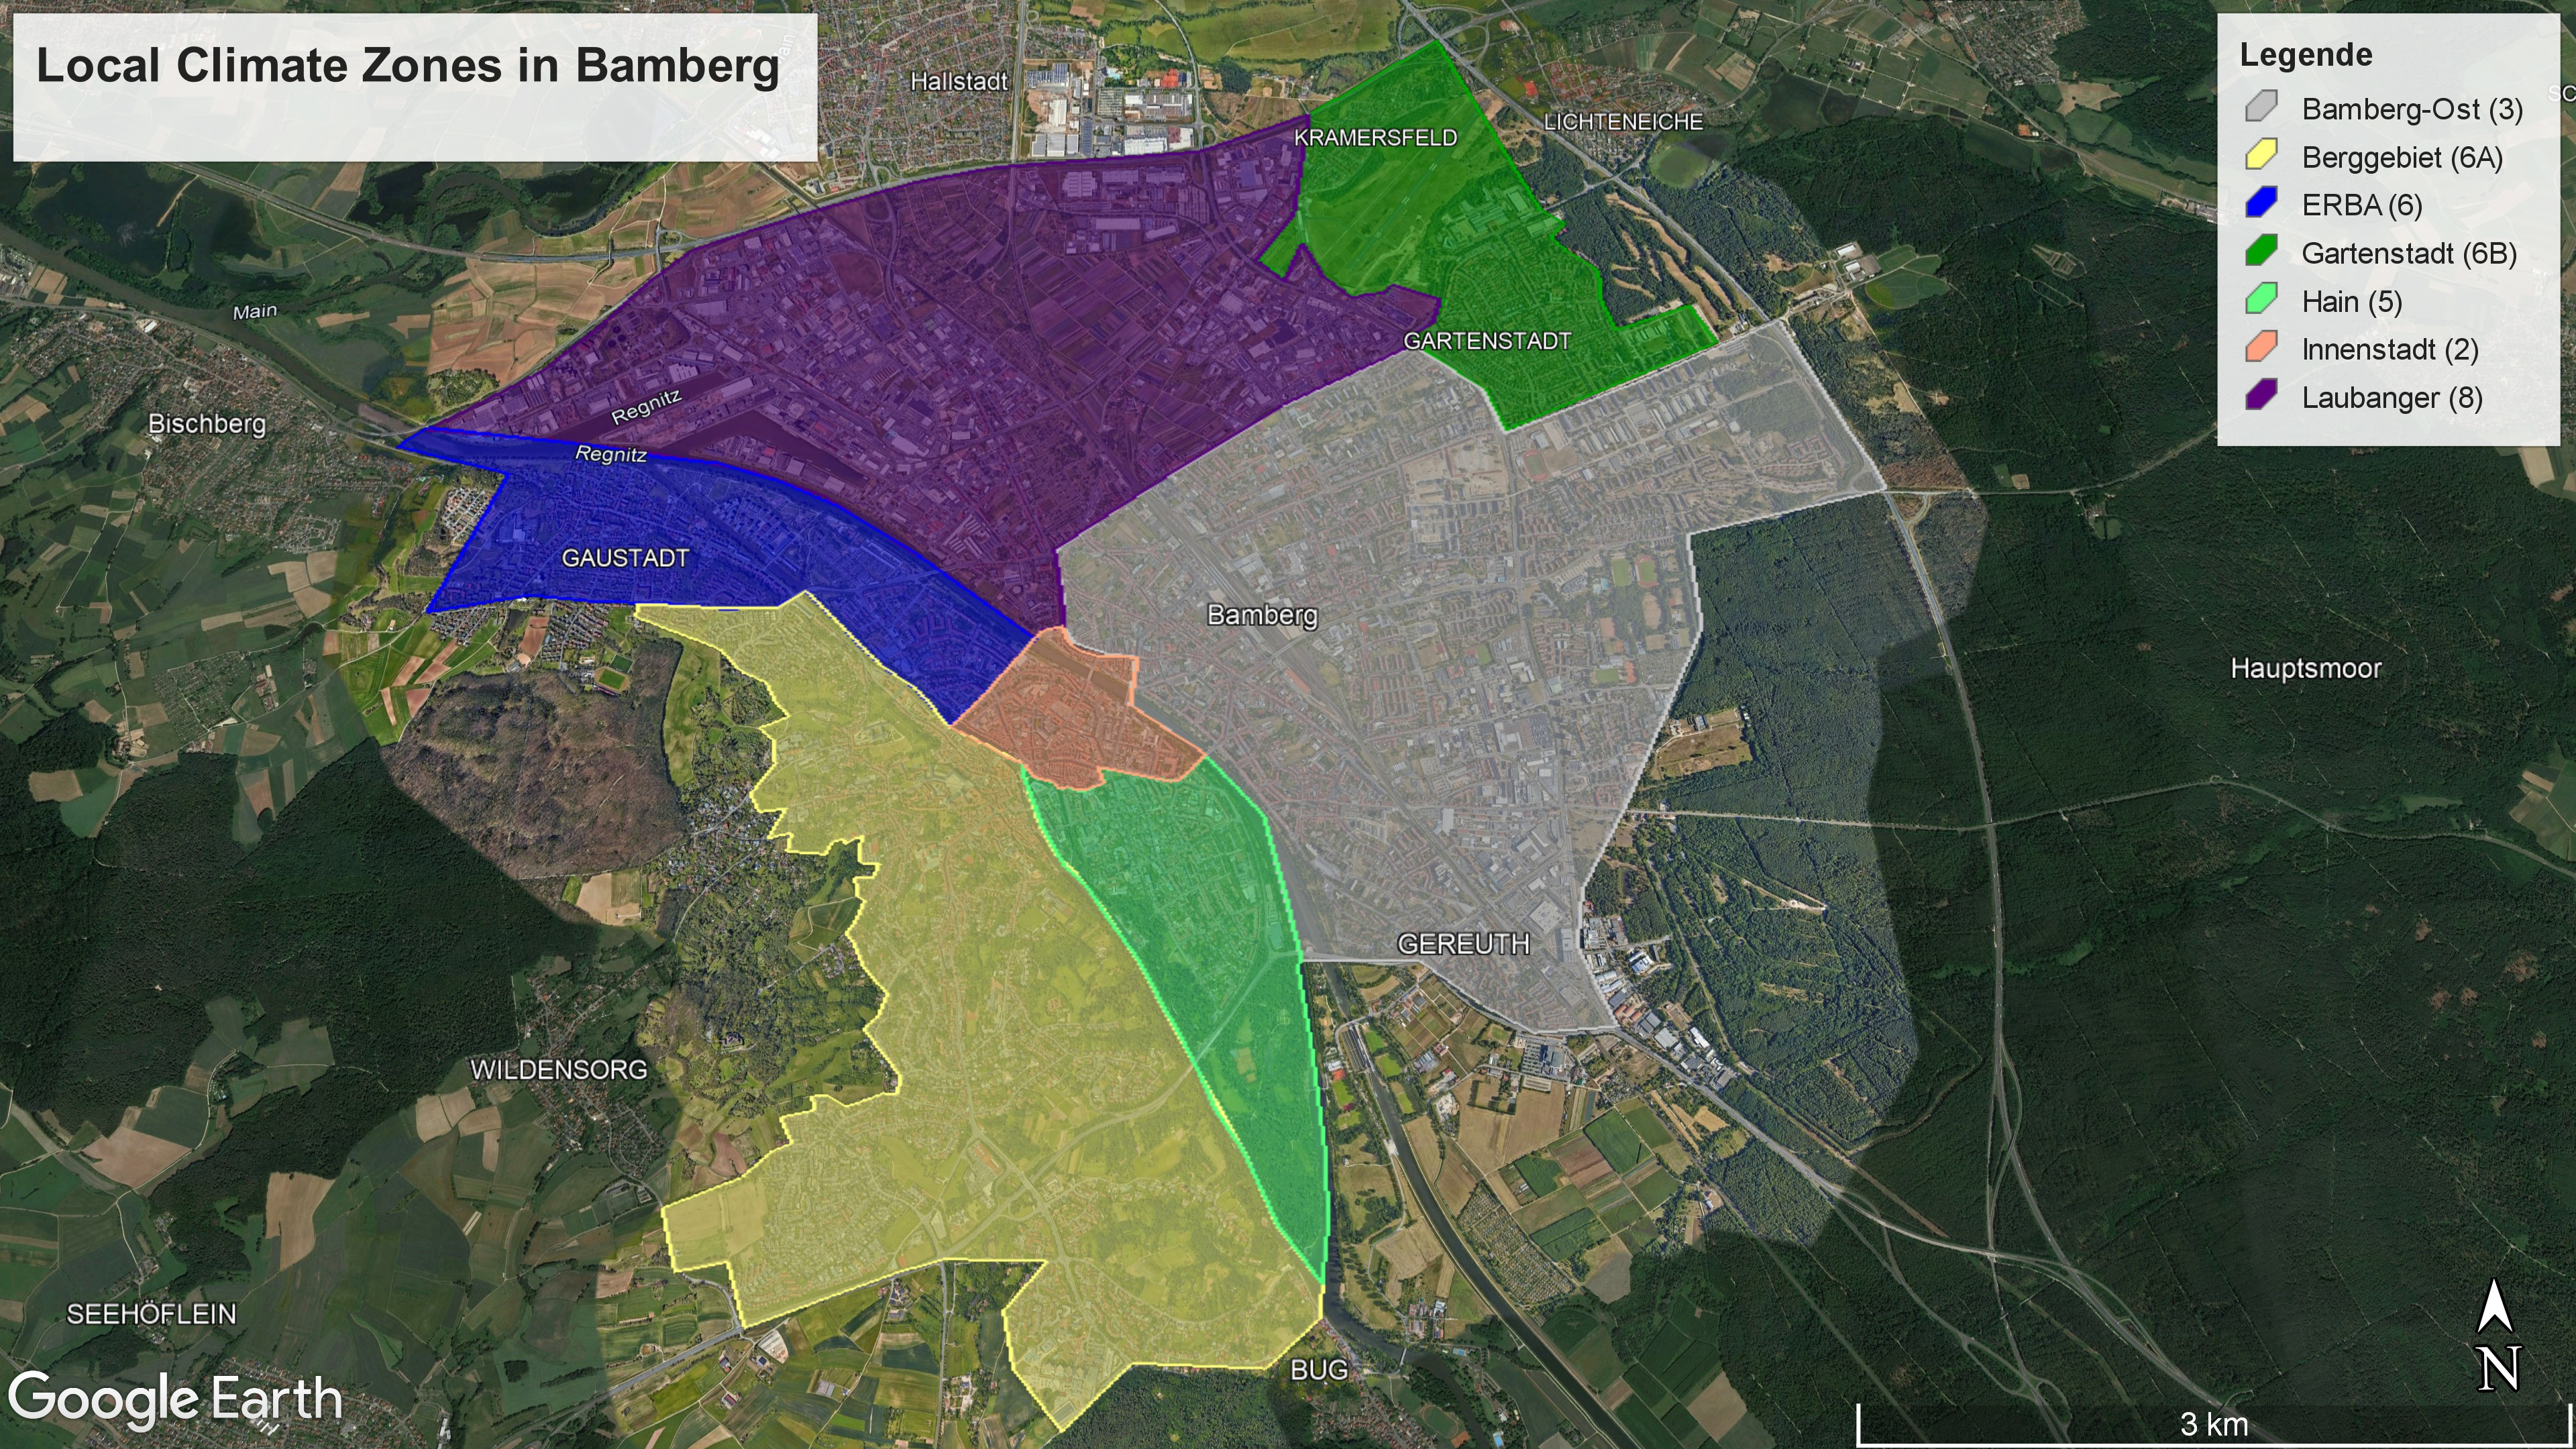
\includegraphics[width=1\textwidth]{figures/lcz.jpg}
    \decoRule
    \caption[LCZ in Bamberg]{Die sechs \ac{LCZ} in Bamberg (eigene Darstellung, basierend auf \cite{stewart2012local,oke2004initial})}
    \label{fig:lcz}
\end{figure}

Durch die Unterteilung der Stadt Bamberg in \ac{LCZ} ist es möglich, die Auslesungen der Wetterstationen und die Unterschiede der Messwerte in den einzelnen Gebieten nachvollziehen und damit besser analysieren zu können. \\ In der Stadt selbst sind Wetterstationen\sidenote{Die genaue Anzahl der Sensoren ist unbekannt, da nicht alle öffentlich einsehbar sind (Stand Oktober 2023: 42 Wetterstationen einsehbar} verteilt, die jeweils die Temperatur und Luftfeuchtigkeit am entsprechenden Standort messen. Auf der Wetterkarte von Netatmo\sidenote{\url{https://weathermap.netatmo.com/}} sind diese Auslesungen von öffentlichen Netatmo-Wetterstationen einsehbar.

\subsection{Identifikation der Stakeholder}
\label{sec:stakeholder}
In diesem Abschnitt der Arbeit werden die Stakeholder identifiziert, dessen Bedürfnisse und Ansprüche durch die Entwicklung des interaktiven Werkzeuges befriedigt werden sollen. Diese werden im Folgenden vorgestellt:

\paragraph{Der Bürgerverein Bamberg Mitte e.V.}
Bei dem \ac{BVM} handelt es sich um einen Bürgerverein in der Stadt Bamberg, welcher 1905 gegründet wurde und mit zahlreichen Projekten\sidenote{\url{https://bvm-bamberg.de/de/projektseiten/projekte-und-aktivitaeten/}} und durch das Praktizieren von Bürgerbeteiligung die Stadt Bamberg, vor allem in Hinblick auf die Stadtplanung und des Umwelt- und Denkmalschutzes, mitgestaltet\sidenote{\url{https://bvm-bamberg.de/de/buergerverein/unser-verein/}}.

Eines dieser Projekte ist das \enquote{Klimamessnetz auf der Bamberger Inselstadt}. Hier wird seit Anfang 2022 mithilfe von insgesamt neun smarten Netatmo-Wetterstationen\sidenote{\url{https://shop.netatmo.com/de-de/weather/smart-weather-station/weatherstation}} (Stand: 21. Oktober 2023) ein Klimamessnetz im Bamberger Zentrum zum Messen der Temperatur und Luftfeuchtigkeit an den entsprechenden Standorten\sidenote{Standorte der smarten Wetterstationen (\ac{LCZ}): Steinertstraße (Innenstadt), Lange Straße (Innenstadt), Am Weidenufer (ERBA), Holzmarkt (Innenstadt), Promenadestraße (Innenstadt), Wetzelstraße (ERBA), Fischerei (Innenstadt), Frauenstraße (Innenstadt) und Hainstraße (Hain)} aufgebaut. \\ Aus den Messungen der Wetterstationen ergibt sich, dass sich die Bamberger Innenstadt im Vergleich zu anderen \ac{LCZ} kaum abkühlt und die Temperaturen sich häufig von der offiziellen Station des \ac{DWD} unterscheiden (vgl. Webauftritt\sidenote{\url{https://bvm-bamberg.de/de/projektseiten/klima/}} des \ac{BVM}). Dies ist auch darauf zurückzuführen, dass das Fehlen von Bäumen und Grünflächen als Charakteristika eines \enquote{Compact mid-rise} ausschlaggebend für das Aufwärmen der Innenstadt ist: Ein Team von Geoökologen der Universität ETH Zürich hat in einer Studie gezeigt, dass Grünanlagen mit Bäumen in Städten zu einem Kühlungseffekt führen \cite{bastin2019global}. Dieser Effekt entsteht durch die Tatsache, dass Bäume durch ihre Wurzeln mehr Wasser aufnehmen können, welches im Umkehrschluss an trockenen und heißen Tagen verdunsten und so zu einer Abkühlung führen kann \cite{bastin2019global}. \\ Wie in Kapitel \ref{sec:methodologyrequirements} bereits erläutert, trifft sich der \ac{BVM} in regelmäßigen Abständen zum Analysieren der Auslesungen der Wetterstationen und Diskutieren von Maßnahmen, die zur Abkühlung der Innenstadt beitragen können. Durch die Teilnahme an diesen Treffen und die daraus resultierenden Gespräche mit den Mitgliedern des \ac{BVM} wurde in Erfahrung gebracht, dass das grundlegende Ziel des Vereins ist, Führungspersonen (z.B. in der Politik, Stadtplanung, Ämtern etc.) durch die Auslesungen der Wetterstationen zu sensibilisieren und damit zu einer Verbesserung der Lebensqualität durch das Erreichen des Kühlungseffektes in der Stadt Bamberg beizutragen. Dies soll ihrer Ansicht nach durch das Reduzieren von Parkplätzen (zum Minimieren von stehen gelassenen Autos) und Straßen für Autos erreicht werden, sodass für die neu geschaffenen Flächen Bäume und Grünflächen gepflanzt werden können.

\paragraph{Die Domänenexpert*innen}
Als Domänenexpert*innen werden in dieser Arbeit Personen definiert, die durch ihre Expertise und Erfahrung in einer Domäne wichtige Einblicke und Informationen, die über die Literatur hinausgehen, zu einem Projekt beitragen können. Sowohl für dieses Projekt, als auch für das Projekt des \ac{BVM} fungiert hier Prof.\ Dr.\ Thomas Foken\sidenote{\url{https://www.micrometeorology.de/}}, der durch seine Professur für Mikrometeorologie an der Universität Bayreuth langjährige Erfahrung in der (Mikro-)Meteorologie und der Klimaforschung besitzt. Durch die Teilnahme Prof.\ Dr.\ Fokens an den regelmäßigen Treffen mit dem \ac{BVM} ist es möglich gewesen, Erläuterungen und Definition der (Mikro-)Meteorologie zu erhalten, sodass erste Fokusse der Arbeit gesetzt werden konnten: \\ Einer dieser Punkte sind die sogenannten \enquote{Tropennächte}\sidenote{Nächte, in denen die minimale Temperatur zwischen 18 und 6 Uhr UTC mindestens 20°C betragen hat \cite{TropennachtDWD}} in Deutschland gewesen, die den Analysen des Professors nach eine deutliche Steigung in den letzten Jahren aufweisen. Dieser Aspekt ist insofern gefährlich für den Menschen, da der Körper des Menschen durch eine solche Hitzebelastung auf eine besondere Weise beansprucht wird und Probleme, die sich auf das Herz-Kreislaufsystem des Menschen auswirken, auftreten können \cite{Umweltbundesamt2023Hitze}
Tropennächte bieten sich insofern als guter Messwert an, da diese Kennzeichen für Hitzewellen in relativ kühleren Regionen der Welt (\textit{hier:} Deutschland) und für ihre geringe Frequenz eigentlich eine Ausnahmeerscheinung repräsentieren sollten TODO HIER ZITAT. [...]

\paragraph{Der \ac{MOBI-Lehrstuhl}}
Der \ac{MOBI-Lehrstuhl}\sidenote{\url{https://www.uni-bamberg.de/mobi/}} ist ein Lehrstuhl, welcher 2014 in der Fakultät Wirtschaftsinformatik und Angewandte Informatik an der Otto-Friedrich-Universität Bamberg angelegt wurde. Die Leitung übernimmt Prof.\ Dr.\ Daniela Nicklas, welche gleichzeitig die Betreuerin dieser Arbeit darstellt. Der Lehrstuhl beschäftigt sich insbesondere mit den \enquote{Fragen des Datenmanagements für mobile Systeme, Datenstrommanagement/komplexe Ereignisverarbeitung und der Unterstützung sensorbasierter Anwendungen, unter anderem im Bereich Smart Cities}. Die Hauptansprechpartner*innen im Rahmen dieser Arbeit sind Prof.\ Dr.\ Daniela Nicklas, Leonie Ackermann und Aboubakr El Hacen Benabbas gewesen. \\ Der MOBI-Lehrstuhl hat ebenfalls an den regelmäßigen Treffen des \ac{BVM} zusammen mit Prof.\ Dr.\ Thomas Foken teilgenommen, sodass hier zusätzlich die Möglichkeit bestanden hat, Erfahrungen und Wissen aus dem Bereich der Informatik, der Datenverarbeitung und notwendige Schritte zum Entwickeln eines interaktiven Werkzeuges zu erhalten. Im gemeinsamen Austausch wurden Anforderungen ausgearbeitet, die sowohl für das \ac{BVM} und die Domänenexpert*innen in Hinblick auf die Auslesungen der Wetterstationen und die damit verbundenen Analysen der Sensordaten, als auch für den \ac{MOBI-Lehrstuhl} in Hinblick auf die technische Umsetzung relevant, aber auch realistisch sind.

\paragraph{Weitere Stakeholder}
Da eine Stadt selbst nicht als Stakeholder identifiziert werden kann, weil eine solche keine eigene Entscheidungs- bzw. Handlungseinheit darstellt, sollte Bamberg selbst trotzdem in diesem Abschnitt erwähnt werden. Dies ist darauf zurückzuführen, dass im Idealfall die eingesetzte Software Regierungsbehörden, Verwaltungen oder ähnliche Organisationen der Stadt erreichen kann und im Idealfall die Auswirkungen dieser Sache Bürger*innen, Unternehmen oder andere Interessensgruppen innerhalb der Stadt betreffen. Allerdings hat zum Zeitpunkt der Anforderungsanalyse weder mit der Stadt Bamberg, noch mit den Bürger*innen ein Austausch stattgefunden, sodass diese als indirekter Stakeholder erwähnt, aber weiterführend in dieser Arbeit nicht betrachtet werden.

Die in diesem Kapitel erläuterten Stakeholder wurden zum Zeitpunkt der Anforderungsanalyse identifiziert. Eine Limitierung auf diese Stakeholder ist aber nicht gegeben, sodass im Laufe der Arbeit oder in der Zukunft weitere Stakeholder identifiziert und in die Anforderungsanalyse aufgenommen werden können.
% \subsection{Das Bamberger Klimamessnetz als Grundlage der Sensordaten}

\section{Anforderungen}
In diesem Abschnitt der Arbeit werden die Anforderungen an das interaktive Werkzeug definiert. Diese werden in den folgenden Abschnitten erläutert und in einer Tabelle (vgl. TODO HIER TABELLE) zusammengefasst.

\subsection{Erfassung}
Die folgenden Anforderungen sind bei den Treffen mit den Stakeholdern erfasst worden. Eine Unterscheidung zwischen funktionalen\sidenote{Funktionale Anforderungen bestimmen spezifische Funktionen, Operationen oder Aufgaben, die eine Applikation (oder ihre Komponenten) ausführen muss, um die Bedürfnisse der Stakeholder zu erfüllen. Wenn das System die funktionalen Anforderungen nicht erfüllt, dann ist eine grundlegende Funktionalität des Systems nicht gegeben \cite{Puzhevich2021}} und nicht-funktionalen\sidenote{Nicht-funktionale Anforderungen beschreiben Qualitätsmerkmale und Leistungsaspekte einer Applikation (oder ihrer Komponenten). Dabei handelt es sich nicht um spezifische Funktionen, sondern um die Art und Weise, wie diese Funktionen erbracht werden sollen \cite{Puzhevich2021}} Anforderungen wird hierbei getroffen, um diese besser zu strukturieren und priorisieren zu können. Eine Übersicht aller erfassten Anforderungen ist in der Tabelle \ref{sec:requirements_table} zu finden. Im weiteren Verlauf dieses Unterkapitels werden für eine citizen-science Anwendung typische\sidenote{Unterschieden wird dieser Aspekt dadurch, was eine typische Anwendung mit einem Crowdsensing-Ansatz von einer Anwendung ohne diesen unterscheidet (z.B. Login/Registrierung vs. Messen von Sensordaten in Echtzeit)} Anforderungen in der folgenden Form näher erläutert:

\textbf{Name der Anforderung (FR/NFR)}: Beschreibung und Begründung der Anforderung (\textit{Passform-Kriterium}; Priorität, wobei 1 die geringste und 5 die höchste Priorität darstellt)

\begin{enumerate}
    \item \textbf{Einsehen der Sensordaten in Echtzeit (FR)}: Die Nutzer*innen sollen die Möglichkeit haben, die Sensordaten in Echtzeit einsehen zu können. Dadurch soll es möglich sein, die Temperatur und Luftfeuchtigkeit an den entsprechenden Standorten zu betrachten und zu analysieren (\textit{Eine interaktive Karte mit den verschiedenen Stationen ist einsehbar und jede Station wird mit dem aktuellen Messwert der Temperatur und Luftfeuchtigkeit angezeigt}; 5)
    \item \textbf{Chatfunktionalität einer Station (NFR)}: Nach Wahl einer Station soll es möglich sein, eine Information an der gewählten Station zum gewählten Zeitpunkt zu hinterlassen. Der Grund dafür ist, dass Nutzende erkannte Anomalien eines ausgewählten Sensors erklären können (\textit{Textbox zur Eingabe des Chats erscheint nach Wahl einer Station und Zeitpunkt, Eingabe wird dauerhaft gespeichert}; 4)
    \item \textbf{Qualitätskontrolle der Sensordaten (NFR)}: Die Sensordaten sollen vor der Visualisierung mithilfe eines Algorithmus auf ihre Qualität überprüft und gefiltert werden. Dies soll durch das bestmögliche Entfernen von Ausreißern und das Ersetzen von fehlenden Werten erfolgen. Begründet ist dieser Aspekt dadurch, dass Fehler und Anomalien in den Sensordaten zu einer Verfälschung der Ergebnisse führen können (\textit{Qualitätskontrolle ist vor der Visualisierung der Sensordaten implementiert}; 4)
    \item \textbf{Speichern von Einstellungen (NFR)}: Die Einstellungen, die von den Nutzenden getätigt werden, sollen gespeichert werden, sodass diese beim nächsten Besuch der Anwendung wiederhergestellt werden können. Dadurch soll eine personalisierte Nutzung der Anwendung ermöglicht werden (\textit{Einstellungen werden in der Datenbank gespeichert und beim nächsten Besuch der Anwendung wiederhergestellt}; 4)
    \item \textbf{Vergleiche zwischen Stationen (NFR)}: Für Nutzende soll es möglich sein, mehrere Stationen auszuwählen und die Sensordaten der ausgewählten Stationen miteinander zu vergleichen, sodass Aussagen über das Klima, vor allem im Vergleich zwischen den \ac{LCZ}, getroffen werden können (\textit{Auswahl von mehreren Stationen ist zu gewünschten Zeitpunkten bzw. -fenstern ist möglich}; 4)
    \item \textbf{Heatmap (FR)}: Durch das Klicken eines Buttons soll es möglich sein, eine Heatmap der Temperatur und Luftfeuchtigkeit zu der eingeblendeten Karte der Stadt Bamberg zu aktivieren. Dadurch sollen Unterschiede zwischen den verschiedenen \ac{LCZ} sichtbar gemacht werden, um darauf basierend Rückschlüsse ziehen zu können (\textit{Heatmap wird durch Klicken eines Buttons aktiviert und die Temperatur und Luftfeuchtigkeit wird durch Farben dargestellt}; 3)
    \item \textbf{Einstellen des Zeitfensters für Stationen (NFR)}: Mithilfe verschiedener Auswahlmöglichkeiten soll die Anzeige der Auslesungen für die Stationen so manipuliert werden können, dass Auslesungen für unterschiedliche Zeiträume und -punkte angezeigt werden können. Dadurch sollen die Auslesungen im Verlauf der Zeit betrachtet werden können (\textit{Auswahlmöglichkeiten für die Anzeige der Auslesungen sind vorhanden, gewähltes Zeitfenster manipuliert entsprechend die Anzeige der Auslesungen}; 3)
    \item \textbf{Ein- und Ausblenden von Stationen (NFR)}: Es soll die Möglichkeit gegeben werden, einzelne (oder alle) Stationen ein- und auszublenden. Dadurch sollen nur für die Nutzenden relevante Stationen angezeigt werden, sodass eine Übersichtlichkeit auf der Karte ermöglicht wird (\textit{Ein- und Ausblenden von Stationen ist durch Button oder Klick auf entsprechende Stationen möglich}; 3)
    \item \textbf{Vordefinierte Standardsichten (NFR)}: Es sollen vordefinierte Standardsichten existieren, die Nutzende anklicken können, um entsprechende Ansichten auf der Karte zu erhalten. Dadurch können allgemein relevante Einstellungen, wie z.B. Sommertage, Tropennächte etc. schnell abgerufen werden (\textit{Vordefinierte Standardsichten sind vorhanden und können durch Klick auf entsprechende Buttons aktiviert werden}; 3)
    \item \textbf{Einsehen der eigenen Chats (NFR)}: Es soll die Möglichkeit geben, die eigenen Chats in denen die Nutzenden involviert sind, einzusehen. Dadurch soll eine Übersichtlichkeit über die eigenen Chats ermöglicht werden (\textit{Eigene Chats im Bereich \enquote{Mein Bereich} einsehbar}; 2)
    \item \textbf{Hinzufügen von Favoriten (NFR)}: Es soll die Möglichkeit geben, Stationen als Favoriten zu markieren, sodass diese in einem eigenen Bereich gespeichert werden können. Dadurch soll eine Übersichtlichkeit über die eigenen Favoriten ermöglicht werden (\textit{Favoriten können durch Klick auf entsprechende Stationen hinzugefügt werden und sind im Bereich \enquote{Mein Bereich} einsehbar}; 2)
    \item \textbf{Anzeigen von relevanten Landmarks auf der Karte (NFR)}: Es soll die Möglichkeit geben, (temperatur-)relevante Landmarks auf der Karte anzuzeigen. Diese sollen die ausgelesenen Sensordaten insofern unterstützen, sodass Zusammenhänge zwischen den Standorten der Stationen und den lokalen Gegebenheiten, wie z.B. Wasserbrunnen, Wälder etc. erschlossen werden können (\textit{(Temperatur-)relevante Landmarks sind auf der Karte dauerhaft einsehbar}; 2)
    \item \textbf{Einheitliche Datenverwaltung (NFR)}: Die Daten sollen in einer einheitlichen Datenbank verwaltet werden, da diese zum aktuellen Stand an unterschiedlichen Orten vorliegen und eine Übersicht erschweren (\textit{Daten liegen auf einer Datenbank vor und ein Zugriff auf diese ist möglich}; 1)
\end{enumerate}

Eine Limitierung der Anforderungen auf diese genannten ist nicht gegeben. Es ist möglich, dass im Laufe der Arbeit weitere Anforderungen hinzukommen oder bestehende Anforderungen angepasst werden.

\subsection{Priorisierung}
Die Priorisierung der Anforderungen erfolgt anhand der \textit{MoSCoW}-Methode\sidenote{MoSCoW ist ein Akronym für \textit{Must have, Should have, Could have, Won't have} und wird verwendet, um die Priorität von Anforderungen zu bestimmen \cite{clegg1994case}}. Eine Priorisierung erfolgt dabei durch die Abstimmung mit den Stakeholdern, wobei die Priorität anhand der folgenden Kriterien bestimmt wird:

\begin{itemize}
    \item \textbf{Must have (5)}: Anforderungen, die als \enquote{Must have} klassifiziert werden, sind essentiell für das Projekt und müssen umgesetzt werden, da diese für die Stakeholder von hoher Bedeutung sind.
    \item \textbf{Should have (4)}: Anforderungen, die als \enquote{Should have} klassifiziert werden, sind wichtig für das Projekt und sollten umgesetzt werden, da diese für die Stakeholder von hoher Bedeutung sind.
    \item \textbf{Could have (3-2)}: Anforderungen, die als \enquote{Could have} klassifiziert werden, sind wünschenswert für das Projekt und können umgesetzt werden, da diese für die Stakeholder von mittlerer Bedeutung sind.
    \item \textbf{Won't have (1)}: Anforderungen, die als \enquote{Won't have} klassifiziert werden, sind nicht relevant für das Projekt und werden nicht umgesetzt, da diese für die Stakeholder von geringer Bedeutung sind.
\end{itemize}

Unter den Kategorien \enquote{Must have} und \enquote{Should have} finden sich unter anderem auch Anforderungen, die für ein citizen-science Projekt essenziell sind, da dieser Aspekt den Fokus dieser Arbeit repräsentiert. Die Kategorien \enquote{Could have} und \enquote{Won't have} beinhalten Anforderungen, die bedeutend und wünschenswert für das Projekt sind, aber nicht zwingend umgesetzt werden müssen. 

\subsection{Analyse}
Aufgrund der Tatsache, dass unter den Stakeholdern auch Domänenexpert*innen, für sowohl die technische Umsetzung als auch für die Domäne der (Mikro-)Meteorologie lokalisiert werden können, befinden sich alle aufgestellten Anforderungen in einem realistischen Rahmen, wenn lediglich die allgemeine Realisierbarkeit betrachtet wird. Inwiefern die Anforderungen in der vorgegebenen Zeit umgesetzt werden können, wird bereits in Kapitel \ref{sec:umsetzung} erläutert. \\ Um den Crowdsensing-Ansatz dieser Arbeit zu erfüllen, und Rückschlüsse auf einen Mehrwert durch die Nutzung dieses Ansatzes zu ziehen, müssen entsprechende Anforderungen existieren und höher priorisiert sein. Dies wird erreicht durch die Anforderungen 

\begin{itemize}
    \item Chatfunktionalität einer Station
\end{itemize}

mit dessen Implementierung Nutzende aktiv Anomalien erkennen, markieren und im weiteren Verlauf eine Erklärung für den Ursprung dieser zu finden. Bevor es zu diesem Schritt kommen kann, muss die Umgebung für diesen Prozess gebaut werden. Dafür benötigt man die Anforderungen 

\begin{itemize}
    \item Einsehen der Sensordaten in Echtzeit
    \item Vergleiche zwischen Stationen
    \item Einstellen des Zeitfensters für Stationen
\end{itemize}

sodass eine Grundlage für das Verfassen einer Annotation gegeben ist. Um die Qualität der vorliegenden Daten und der Nutzenden-Erfahrung zu steigern, werden die Anforderungen 

\begin{itemize}
    \item Qualitätskontrolle der Sensordaten
    \item Speichern von Einstellungen
    \item Heatmap
    \item Ein- und Ausblenden von Stationen
    \item Vordefinierte Standardsichten
    \item Hinzufügen von Favoriten
    \item Anzeigen von relevanten Landmarks auf der Karte
    \item Einheitliche Datenverwaltung
\end{itemize}

aufgestellt. Aus dieser Aufzählung wird deutlich, dass das Ziel des Projektes, und damit des Crowdsensing-Ansatzes, klar durch das Vorhandensein einer Anforderung (Chatfunktionalität einer Station) definiert ist. Alle anderen aufgestellten Anforderungen stellen dabei nur Notwendigkeiten dar, dieses Ziel zu erreichen oder die Qualität des Endproduktes zu steigern. \\ Aufgrund dessen befinden sich die aufgestellten Anforderungen ebenfalls in einem validen Rahmen. Dies ist zusätzlich darauf zurückzuführen, dass das Projekt iterativen Prozessen unterliegt, sodass die Anforderungen nach jeder Iteration in Form der regelmäßigen Treffen mit den Stakeholdern angepasst werden können. Paradoxe, nicht-realisierbare oder den Rahmen sprengende Anforderungen werden mit den Stakeholdern evaluiert, sodass entsprechende Lösungen gebildet werden oder diese angepasst werden können, um Validität zu gewährleisten.

Inwieweit die Anforderungen dieses Projekts erfüllt sind, wird in Kapitel \ref{sec:requirements_evaluation} evaluiert. 

\section{User Stories}
Im folgenden werden TODO: HIER ANZAHL User Stories beschrieben, um die Anforderungen an einem konkreten Beispiel zu repräsentieren. 

\subsubsection{User Story \#1}

\subsubsection{User Story \#2}

\section{Use-Case-Diagramm}
Um auf eine simple Art und Weise aufzuzeigen, was die fertige Softwarelösung können muss, kann ein Use-Case-Diagramm (vgl. Abbildung \ref{fig:usecase_diagram}) eingesetzt werden. In diesem werden die Akteure (\textit{hier:} User und Administrator) und die entsprechenden Anwendungsfälle in Ellipsen dargestellt. Die Beziehungen der einzelnen Anwendungsfälle untereinander, aber auch mit den Akteuren wird durch gerichtete Graphen verdeutlicht. Das Rechteck repräsentiert das System und dessen Grenzen, in welchem sich die einzelnen Anwendungsfälle befinden. 

\begin{figure*}[t]
    \centering
    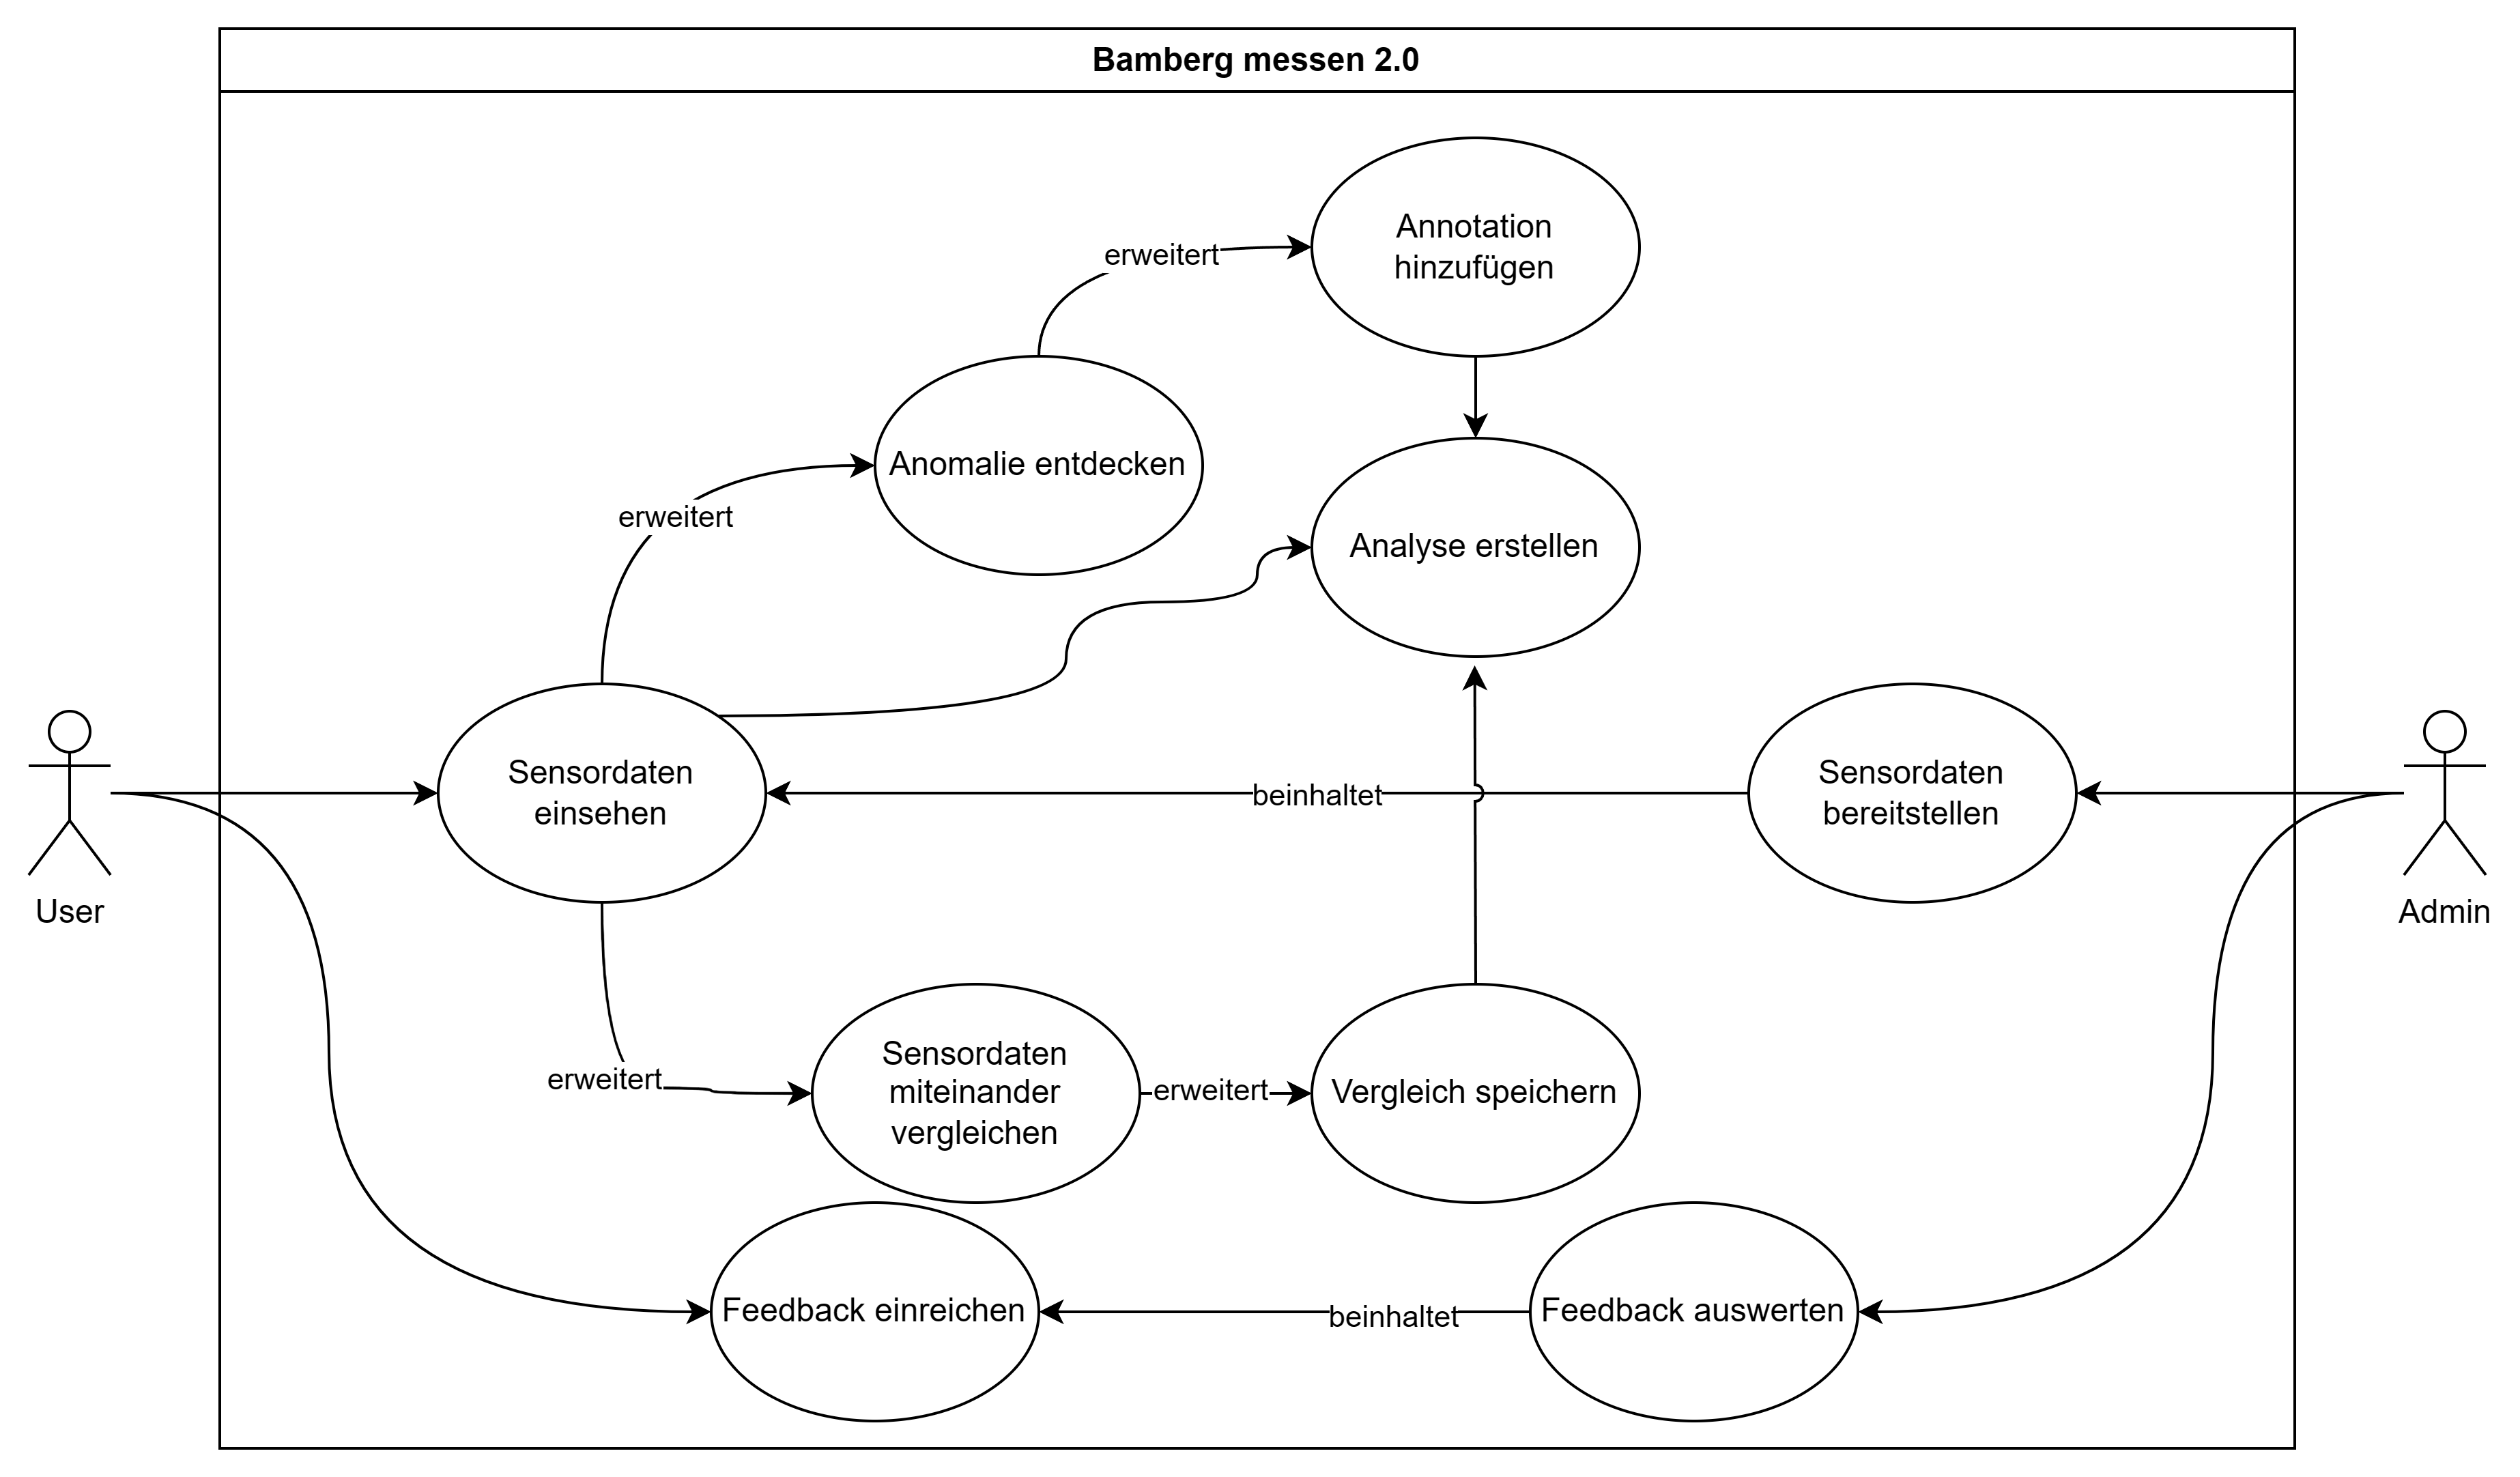
\includegraphics[width=1.5\textwidth]{figures/usecases.png}
    \decoRule
    \caption[Use-Case-Diagramm]{Use-Case-Diagramm}
    \label{fig:usecase_diagram}
\end{figure*}
\chapter{User Stories} % Kapitel zu User Stories
\chapter{Implementierung und Design}
\label{sec:implementation}
In diesem Kapitel der Arbeit wird die Implementierung auf Basis der aufgestellten Anforderungen in Kapitel \ref{sec:requirements} betrachtet. Die Verzeichnisstruktur, auf welche in den folgenden Kapiteln eingegangen wird, ist als Baumstruktur mit Abbildung \ref{fig:dirstructure} gegeben. Die gesamte Applikation befindet sich auf dem Repository im Verzeichnis \texttt{app}. Da die allgemeine Architektur (vgl. Abbildung \ref{fig:architecture}) mithilfe der Containervirtualisierung über Docker aufgebaut ist, wird zunächst dieser Aspekt erläutert. Im Anschluss findet jeweils eine Unterscheidung zwischen der Architektur für das Front-End und das Back-End statt.

\begin{figure*}[t]
    \centering
    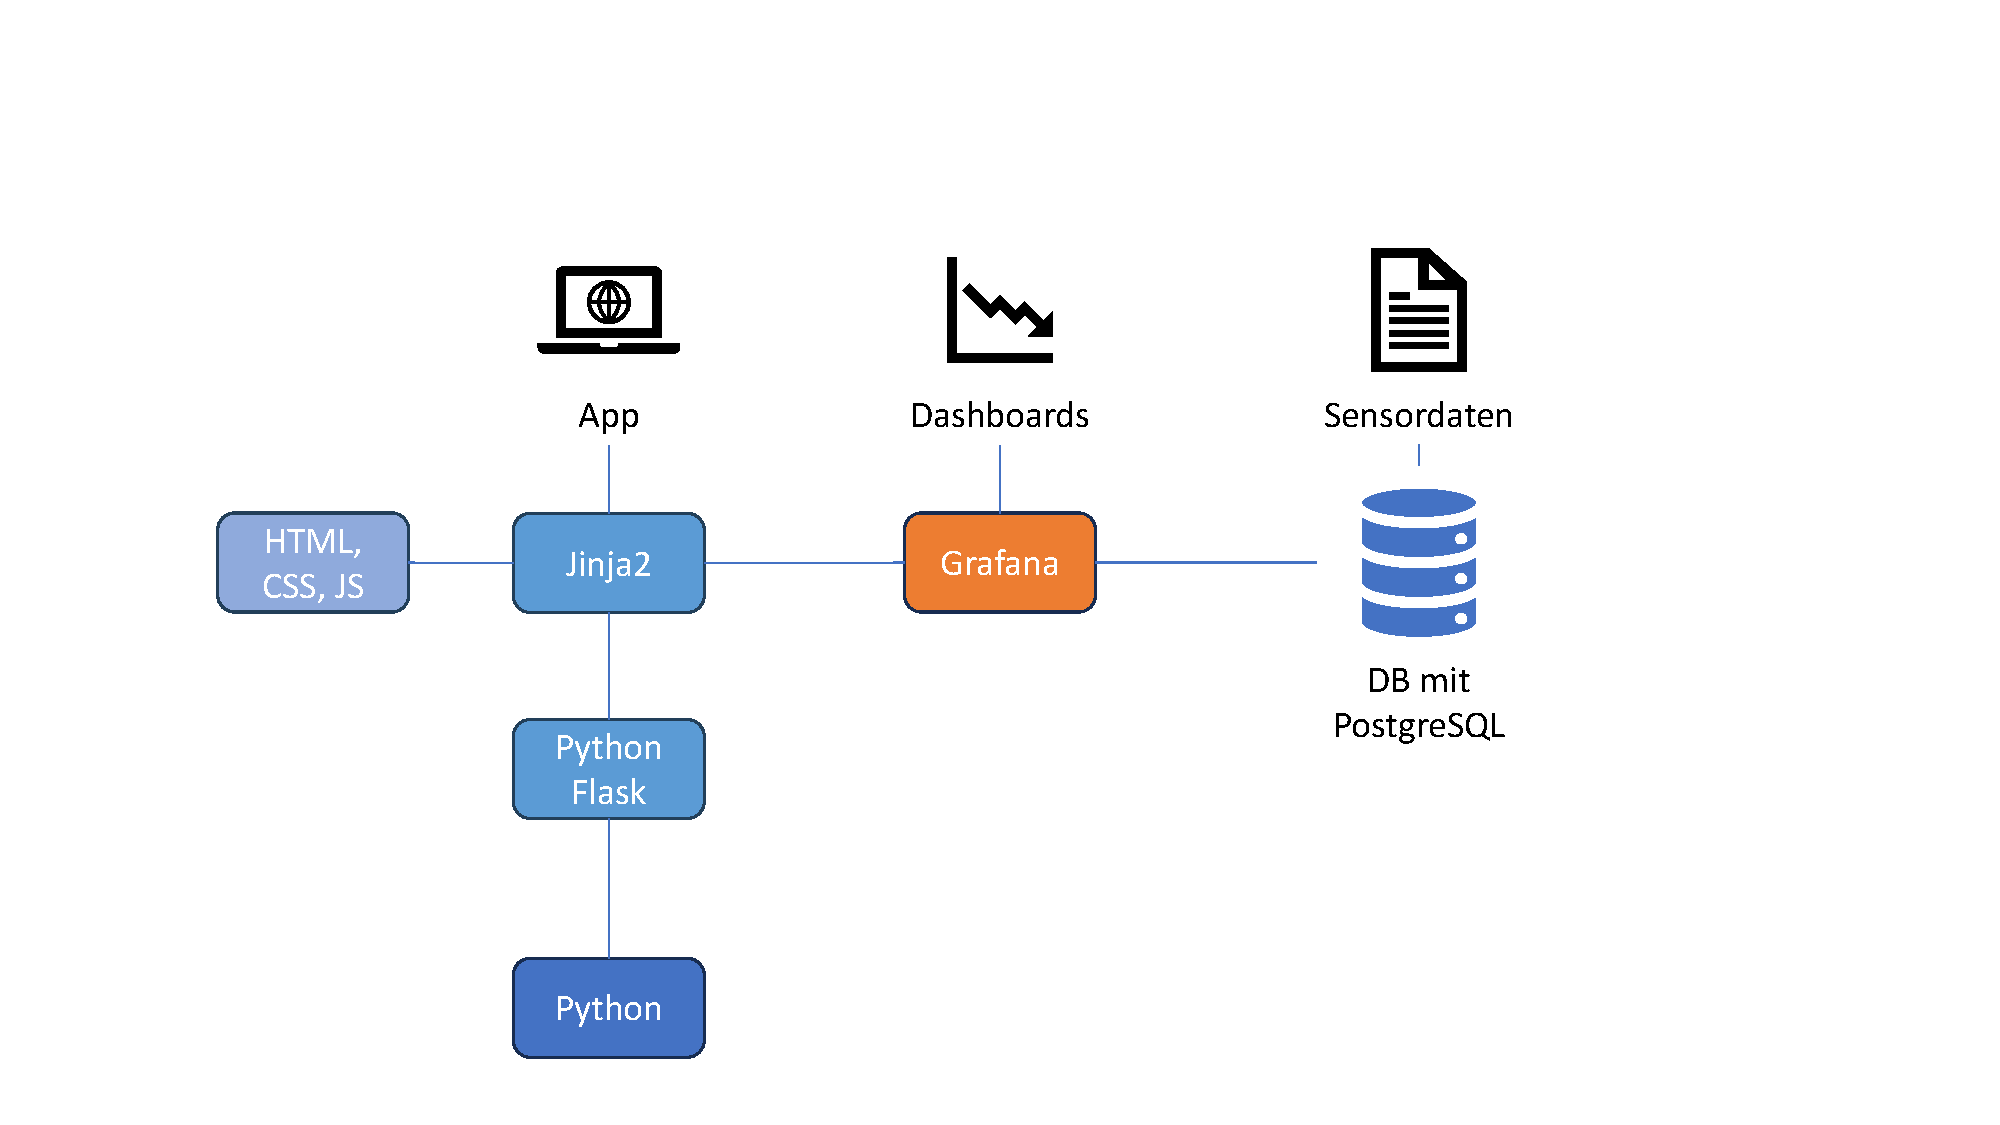
\includegraphics[width=\widefigurewidth]{appendices/Architektur.pdf}
    \caption[Architektur]{Die vorliegende Architektur für die Applikation}
    \label{fig:architecture}
\end{figure*}

\begin{marginfigure}
    \centering
    \begin{adjustbox}{width=\textwidth}
        \begin{tikzpicture}[
                grow=right,
                scale=1.5,
                level 1/.style={sibling distance=2cm},
                level 2/.style={sibling distance=1cm}
            ]
            \node{app}
            child { node {db}
                    child { node {data}}
                    child { node {init.sql}}}
            child { node {grafana}
                    child { node {provisioning}
                            child { node {dashboards}}
                            child { node {datasources}}
                        }
                }
            child { node {web}
                    child { node {static}
                            child { node {css}}
                            child { node {js}}
                            child { node {img}}}
                    child { node {templates}}
                    child { node {index.py}}
                    child { node {requirements.txt}}
                }
            child { node {docker-compose.yml}};
        \end{tikzpicture}
    \end{adjustbox}
    \caption{Die Verzeichnisstruktur der Applikation}
    \label{fig:dirstructure}
\end{marginfigure}

\section{Containervirtualisierung mit Docker}
Aufgrund der Tatsache, dass ein privater Entwickler ein Produktivsystem mit mehreren Komponenten simulieren muss, hat sich der Einsatz Dockers als sinnvoll erwiesen. Docker ist eine Open-Source-Software, die es ermöglicht, Anwendungen mithilfe von Containervirtualisierung zu isolieren. Dabei wird die Anwendung in einem Container ausgeführt, der alle Abhängigkeiten enthält, die für die Ausführung der Anwendung erforderlich sind. Die Container sind dabei leichtgewichtiger als virtuelle Maschinen, da sie den Kernel des Host-Betriebssystems nutzen\sidenote{\url{https://www.docker.com/resources/what-container/}}. Für diese Arbeit sind drei Anwendungen notwendig: eine Python-Flask Instanz für einen Webserver (Port 5000), eine PostgreSQL-Instanz für die Datenbank (Port 5432) und eine Grafana-Instanz (Port 3000) für die Verarbeitung und Visualisierung der Daten aus der Datenbank. Diese drei Anwendungen werden jeweils in einem eigenen Container ausgeführt und einem Netzwerk zugewiesen, um eine Kommunikation zwischen den Containern zu ermöglichen (vgl. Abbildung \ref{fig:dockerarchitecture}). Diese notwendigen Eigenschaften werden in einer \texttt{docker-compose.yml}-Datei definiert. Diese Datei wird von Docker verwendet, um die Container zu erstellen und zu starten. Die \texttt{docker-compose.yml}-Datei befindet sich im Hauptverzeichnis der Applikation.

\begin{figure*}[t]
    \centering
    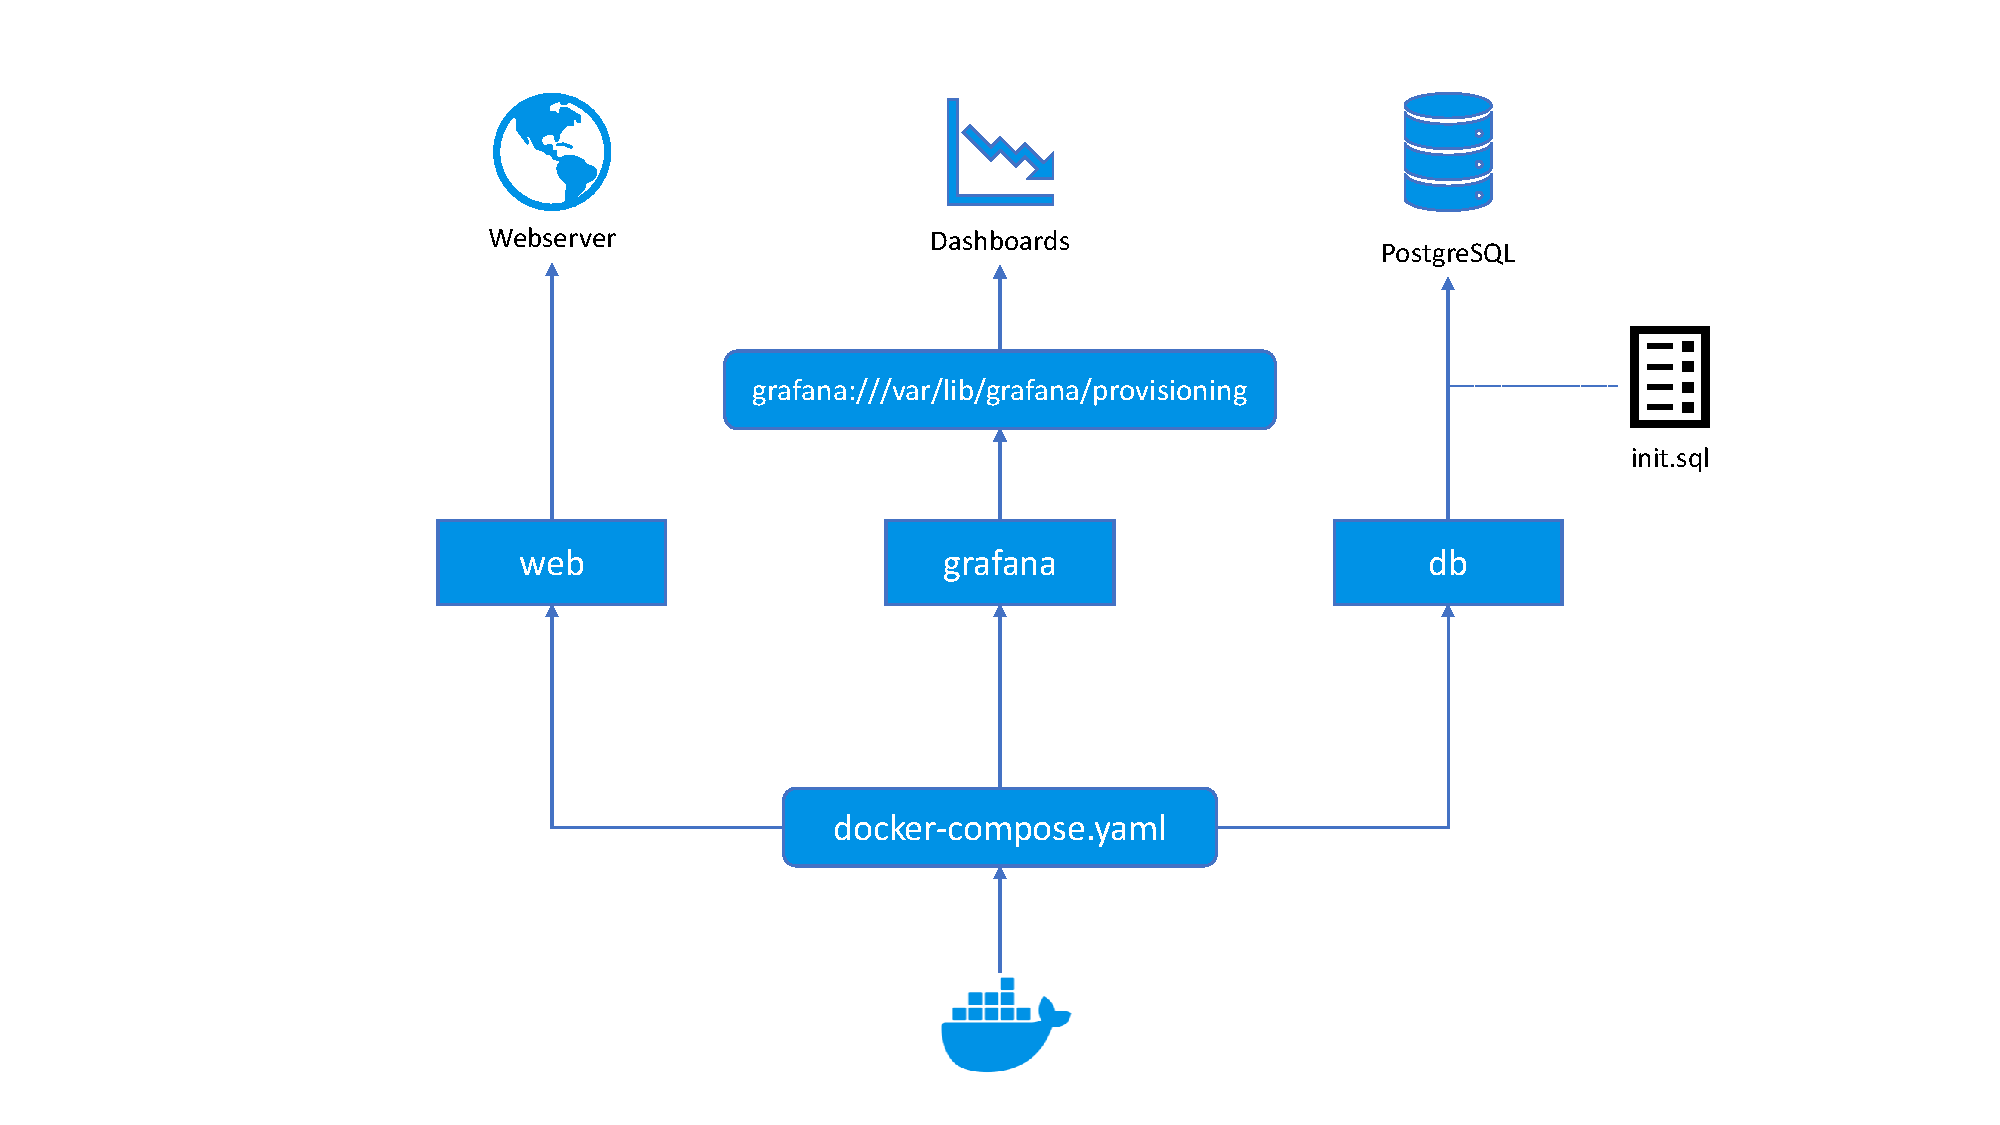
\includegraphics[width=\widefigurewidth]{appendices/Architektur_Docker.pdf}
    \caption[Docker-Architektur]{Die vorliegende Docker-Architektur für die Applikation}
    \label{fig:dockerarchitecture}
\end{figure*}

\section{Architektur für das Front-End}
Das Front-End der Applikation ist mit dem Web-Framework Python-Flask\sidenote{\url{https://flask.palletsprojects.com/}} und den daraus resultierenden Komponenten umgesetzt. Die Wahl, welche Programmiersprache zur Implementierung des Werkzeugs zum Einsatz kommen soll, ist auf Python\sidenote{\url{https://www.python.org/}} gefallen, da es sich um eine leichtgewichtige und einfach zu erlernende Sprache handelt. Zudem ist Python eine der beliebtesten Programmiersprachen\sidenote{\url{https://spectrum.ieee.org/top-programming-languages-2022}} und bietet daher eine umfangreiche Dokumentation zum Umsetzen der individuellen Anforderungen. Flask verwendet als Template-Engine Jinja2\sidenote{\url{https://jinja.palletsprojects.com/}}, mit dessen Hilfe HTML- und JavaScript-Code, als auch CSS-Stylesheets eingebunden werden können. Alle Webserver-Komponenten befinden sich im Verzeichnis \enquote{web}. Innerhalb dieses Verzeichnisses ist folgende Unterteilung vorzufinden:

\begin{itemize}
    \item \textbf{templates} für alle HTML-Dateien, die als Templates für die Jinja2-Engine dienen. In diesem Verzeichnis befindet sich die \texttt{base.html}, welche die Grundlage für alle anderen HTML-Dateien darstellt. In dieser Datei werden alle notwendigen Komponenten wie Stylesheets, JavaScript-Code und die Navigation eingebunden. Die anderen HTML-Dateien erben von dieser Datei und können somit auf die Komponenten zugreifen.
    \item \textbf{static} für alle statischen Dateien, wie CSS-Stylesheets und Bilder (z.B. Favicons für Logos). Auch JavaScript-Dateien werden hier abgelegt um Unterverzeichnisse simpler zu gestalten, obwohl es sich hier um eine dynamische Programmiersprache handelt.
    \item \textbf{index.py} für die Python-Flask-Instanz, die den Webserver darstellt. In dieser Datei werden alle Routen definiert, die der Webserver bereitstellen soll. Das Session- und Cookie-Handling, HTTP-Requests und -Responses und das Logging können ebenfalls in dieser Datei definiert werden.
    \item \textbf{requirements.txt} für alle Python-Abhängigkeiten, die für die Ausführung der Applikation notwendig sind. Diese Datei wird von Docker verwendet, um die Abhängigkeiten zu installieren.
\end{itemize}

Zum Visualisieren und Interagieren der Daten kommt die Open-Source-Software Grafana\sidenote{\url{https://grafana.com/}} zum Einsatz. Mithilfe von Grafana lassen sich Daten aus einer Datenbank abrufen (vgl. \ref{sec:backend}), individuell visualisieren und in Dashboards einpflegen (vgl. Abbildung \ref{fig:grafana}). Zu Visualisierungszwecken befinden sich acht Dashboards in der Sammlung der Bamberger Wetterstationen, wobei es sich bei einem Dashboard um die Zusammenlegung der anderen sieben Wetterstationen handelt, um einen Vergleich zwischen diesen zu ermöglichen. Der Fokus liegt dabei auf der Visualisierung der Temperatur zu einer gegebenen Uhrzeit für jede Wetterstation. Mithilfe von Grenzwerten, die in den Dashboards definiert werden können, lassen sich Temperaturbereiche farblich\sidenote{Die Farbe Blau soll repräsentativ für kalte Temperaturen sein, während die Farbe Rot hohe Temperaturen symbolisieren soll} hervorheben. Der Aspekt des Crowdsensings wird nativ von Grafana durch die Möglichkeit, einen Punkt auf dem Graphen zu markieren und eine Annotation an diese Markierung hinzuzufügen, unterstützt. Diese Annotationen sollen dann durch andere Nutzer*innen des Werkzeuges eingesehen werden können.

Das Front-End bietet mehrere Seiten an, zwischen jenen mithilfe des Routings navigiert werden kann:

\begin{itemize}
    \item \textbf{Home} für die Startseite der Applikation. Hier werden alle Wetterstationen und die definierten \ac{LCZ} auf einer OpenStreetMap\sidenote{\url{https://www.openstreetmap.org/}}-Karte eingeblendet. Auf der rechten Seite haben die Nutzer*innen mithilfe eines Chatfensters die Möglichkeit, sich mit anderen Nutzer*innen zu den Daten auf der Karte auszutauschen.
    \item \textbf{Sensorinspektor} für die Analyse der Daten aus den Bamberger Wetterstationen. Auf dieser Seite werden die Daten aus Grafana mithilfe von iFrames\sidenote{HTML-Tag zum Einbetten von anderen Dokumenten in eine HTML-Datei} eingebunden und durch Filtermöglichkeiten (zu Wetterstationen, Datum und Uhrzeit) mithilfe von Dropdown-Menüs eingeschränkt.
    \item \textbf{Feedback} für die Möglichkeit, Feedback zu der Applikation zu geben. Hier können die Nutzer*innen eine Nachricht hinterlassen und dieser eine Kategorie zuweisen (Fehlermeldung, Änderungsvorschlag oder neues Feature).
    \item \textbf{User} für die Benutzerverwaltung. Hier ist es möglich, sich zu registrieren und anzumelden. Nach der Anmeldung können die Nutzer*innen ihr Profil, ihre Chats und ihr Feedback einsehen.
\end{itemize}

\begin{marginfigure} % [t]: place at top of page (recommended)
    \centering
    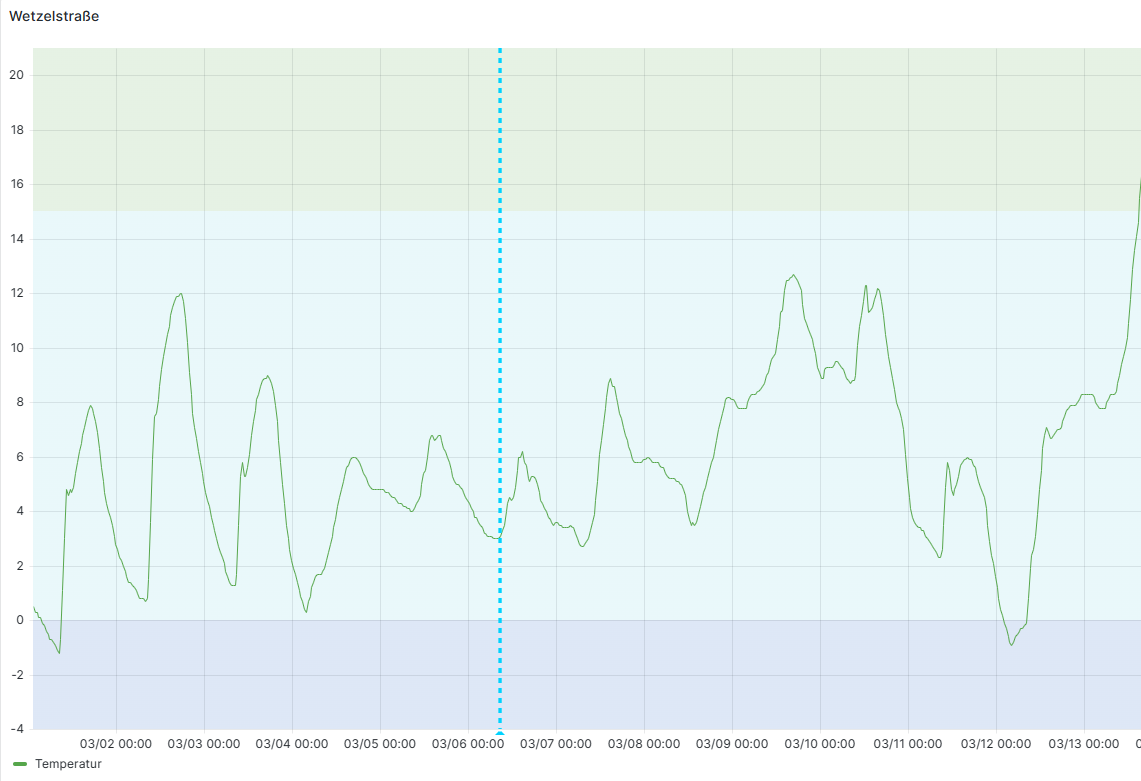
\includegraphics[width=1\textwidth]{figures/grafana.png}
    \decoRule
    \caption[Grafana-Dashboard]{Repräsentatives Grafana-Dashboard mit den Sensordaten aus der Wetzelstraße in Bamberg}
    \label{fig:grafana}
\end{marginfigure}

\section{Architektur für das Back-End}
Das Back-End der Applikation ist mit PostgreSQL\sidenote{\url{https://www.postgresql.org/}} als relationales Datenbankmanagementsystem umgesetzt. Die Wahl, welche Datenbank zum Einsatz kommen soll, ist auf PostgreSQL gefallen, da es sich um Open-Source-Software handelt, eine einfache Einbindung in Grafana möglich ist und PostgreSQL eine umfangreiche Dokumentation zur Verfügung stellt. Zusätzlich entspricht PostgreSQL weitestgehend dem SQL-Standard. \\ Eine Stichprobe\sidenote{Zwischen dem 01. März 2023 und 10. August 2023} der Sensordaten der Wetterstationen in Bamberg wird durch eine parallel laufende Abschlussarbeit am \ac{MOBI}-Lehrstuhl in Form von CSV\sidenote{Comma-separated values, häufiges Dateiformat zum Austausch von Daten}-Dateien zur Verfügung gestellt. Diese Daten werden von Docker Compose beim Starten der Container aus dem Verzeichnis \texttt{db/data} in die Datenbank importiert und durch SQL-Befehle in der Datei \texttt{db/init.sql} in die Datenbank eingefügt (vgl. Abbildung \ref{lst:sqlcode}). \\ Im Anschluss liegt die Tabelle \texttt{stations} in der Datenbank mit folgenden Spalten vor:

\begin{lstlisting}[language=SQL,float=t,
      caption={SQL-Befehle zum Erstellen der Tabelle \texttt{stations} in der Datenbank},label={lst:sqlcode}]
      CREATE TABLE stations (
        id SERIAL PRIMARY KEY,
        p_id INT,
        time TIMESTAMP,
        station VARCHAR(50),
        ta FLOAT,
        lon FLOAT,
        lat FLOAT,
        z INT,
        humidity FLOAT
      );
      
      COPY stations(p_id, time, station, ta, lon, lat, z, humidity) FROM '/data/Bamberg_Stations 01.03.2023to31.03.2023.csv' DELIMITER ';' CSV HEADER;
      COPY stations(p_id, time, station, ta, lon, lat, z, humidity) FROM '/data/Bamberg_Stations 01.04.2023to30.04.2023.csv' DELIMITER ';' CSV HEADER;
      COPY stations(p_id, time, station, ta, lon, lat, z, humidity) FROM '/data/Bamberg_Stations 01.06.2023to30.06.2023.csv' DELIMITER ';' CSV HEADER;
      COPY stations(p_id, time, station, ta, lon, lat, z, humidity) FROM '/data/Bamberg_Stations 01.07.2023to31.07.2023.csv' DELIMITER ';' CSV HEADER;
      COPY stations(p_id, time, station, ta, lon, lat, z, humidity) FROM '/data/Bamberg_Stations 01.08.2023to10.08.2023.csv' DELIMITER ';' CSV HEADER;
      
\end{lstlisting}

\begin{itemize}
    \item \textbf{id} ist notwendig als Primary Key, um die Daten eindeutig zu identifizieren.
    \item \textbf{p\_id} als ID der Wetterstation.
    \item \textbf{time} als Zeitstempel.
    \item \textbf{station} als Name der Wetterstation.
    \item \textbf{ta} als Temperatur in Grad Celsius.
    \item \textbf{lon} als Längengrad.
    \item \textbf{lat} als Breitengrad.
    \item \textbf{z} als Höhe über dem Meeresspiegel.
    \item \textbf{humidity} als Luftfeuchtigkeit in \%.
\end{itemize}

Mit dieser Struktur ist es nun möglich, die Auslesungen der Wetterstationen für einen Zeitpunkt abzufragen. Außerdem bietet die Spalte \texttt{station} die Möglichkeit, nach einer bestimmten Wetterstation zu filtern. Auf diese Weise können die Daten aus der Datenbank in Grafana eingespeist werden.

\label{sec:backend}
\chapter{Diskussion und Evaluation}
Der Hintergrund dieser Arbeit ist durch die Einführung des Crowd\-sen\-sing-Aspekts in die Softwareentwicklung und dessen Auswirkungen auf die Planung, die Software selbst und die Stakeholder gegeben. In diesem Kapitel werden die Ergebnisse dieser Arbeit diskutiert und evaluiert. Dabei wird zunächst darauf eingegangen, inwiefern die Anforderungen aus Kapitel \ref{sec:requirements} erfüllt sind. \\ Anschließend findet eine Evaluation des Projektes statt, in der zuerst die persönlichen Erfahrungen des Autors mit dem Projekt selbst, den Stakeholdern und anschließend unter Zuhilfenahme der Literatur diskutiert werden. Abschließend werden die Limitationen der Arbeit aufgezeigt.
\label{sec:discussion}

\section{Erfüllen der Anforderungen}
\label{sec:requirements_evaluation}
Da dieses Projekt eine zeitliche Limitierung aufweist, ist es grundsätzlich nicht möglich, alle aufgestellten Anforderungen zu erfüllen. Aufgrund dieser Tatsache spielt die Priorisierung eine große Rolle: Diese ermöglicht, eine Reihenfolge der zu erfüllenden Anforderungen einzuhalten und somit die wichtigsten Anforderungen zuerst zu erfüllen. \\ In die Priorisierung fließt gleichzeitig mit ein, den Crowdsensing-Aspekt umzusetzen, sodass die aufgestellten Leitfragen beantwortet werden können. Konkret bedeutet das, dass folgende Anforderungen \textbf{vollständig} umgesetzt sind:

\begin{itemize}
    \item \textbf{Einsehen einer interaktiven Karte:} Eine OpenStreetMap-Karte ist in der Startseite der Applikation eingebettet.
    \item \textbf{Sensordaten als Graphen im Bereich \enquote{Sensorinspektor} anzeigen:} Mithilfe von iFrames über Grafana werden die Sensordaten als Graphen in der Applikation angezeigt.
\end{itemize}

Die folgenden Anforderungen sind \textbf{teilweise} umgesetzt:

\begin{itemize}
    \item \textbf{Einholen der Sensordaten:} Die Sensordaten werden über eine parallel laufende Abschlussarbeit manuell mithilfe von exportierten CSV-Dateien eingeholt. Dieser Schritt sollte automatisiert werden, um die Daten in Echtzeit zu erhalten.
    \item \textbf{Aufbauen einer Datenbank:} Eine grundlegend funktionierende Datenbank ist mithilfe von Docker umgesetzt und kann in die Applikation eingebunden werden. Diese Datenbank ist rudimentär und befindet sich lokal in einem Container auf der Maschine der jeweiligen Nutzer*innen. Ein Datenmodell (z.B. für das User Handling) ist nicht umgesetzt. Ein Hosting in einer Cloud oder einem globalen Server sollte angestrebt werden.
    \item \textbf{Chats für den Bereich \enquote{Sensorinspektor}:} Grundlegend ist es möglich, Annotationen an den Graphen im Bereich \enquote{Sensorinspektor} hinzuzufügen. Hierbei wird zur jeweiligen Position am Graphen zusammen mit dem Zeitstempel eine Texteingabe eingefügt. Allerdings findet eine Speicherung der Eingabe in der Datenbank nicht statt, sodass beim Aktualisieren der Applikation die Annotationen verloren gehen. Eine Anbindung an die Datenbank sollte angestrebt werden.
    \item \textbf{Chats für den Bereich \enquote{Meine Karte}:} Es befindet sich ein Chat-Fenster neben der Karte im Bereich \enquote{Meine Karte}. Hier können Nutzende Chats einfügen, die im Anschluss im Chatfenster angezeigt werden. Allerdings werden diese Chats weder in einer Datenbank gespeichert, sodass bei einer Aktualisierung der Seite alle Chats verloren gehen, noch werden diese mit Daten verknüpft. Andere Nutzer*innen sind ebenfalls nicht in der Lage, die Chats einzusehen. Eine Anbindung an die Datenbank sollte angestrebt werden.
    \item \textbf{Sensoren auf der Karte anzeigen:} Die Sensoren sind mithilfe von Google Earth Pro auf der Karte markiert. Der nächste Schritt ist das Exportieren von KML-Dateien aus Google Earth Pro, um diese mithilfe von OpenLayers in die OpenStreetMap-Karte einzubinden\sidenote{\url{https://openlayers.org/en/latest/examples/kml.html}}. Allerdings ist dieser Aspekt aus zeitlicher Sicht nicht mehr umsetzbar, sodass die Sensoren nicht auf der Karte angezeigt werden.
    \item \textbf{\ac{LCZ} auf der Karte anzeigen:} Durch die identische Vorgehensweise wie bei den Sensoren ist es aus denselben Gründen nicht möglich, die \ac{LCZ} auf der Karte anzuzeigen.
    \item \textbf{Login und Registrierung:} Die Login- und Registrierungsfunktionen sind grundlegend durch die Existenz von entsprechenden Formularen umgesetzt. Allerdings findet keine Verknüpfung mit der Datenbank statt, sodass die Nutzenden sich nicht einloggen können.
    \item \textbf{Manipulieren der Anzeige der Sensordaten:} Im Bereich \enquote{Sensorinspektor} ist es möglich, einen Zeitraum auszuwählen, um die Sensordaten im Graphen zu manipulieren. Allerdings werden die Sensordaten nicht passend manipuliert.
\end{itemize}

Die folgenden Anforderungen sind \textbf{nicht} umgesetzt:

\begin{itemize}
    \item \textbf{Einbinden der \ac{LCZ} in den Bereich \enquote{Sensorinspektor}:} Zum Vergleichen der Daten aus dem Bereich \enquote{Sensorinspektor} ist es zusätzlich hilfreich, die \ac{LCZ} Bambergs bei der Analyse berücksichtigen zu können.
    \item \textbf{Bereich \enquote{Mein Bereich} umsetzen:} Nach erfolgter Registrierung und Login soll es den Nutzenden möglich sein, einen eigenen Bereich einzusehen, in dem die favorisierten Sensoren, beigefügte Chats und Benachrichtigungen angezeigt werden.
    \item \textbf{Aktuelle Auslesungen der Wetterstationen anzeigen:} Die aktuellen Auslesungen der Wetterstationen sollen in der Karte angezeigt werden. Hierfür ist es notwendig, die Daten der Wetterstationen in Echtzeit zu erhalten.
    \item \textbf{Request-Parametrisierung der URL:} Die URL soll die Parameter der Anfrage\sidenote{z.B. \url{http://bamberg-messen.com/station?id=456&timefrom=2023-03-01&timeto=2023-08-01}, um alle Daten der Station mit der ID 456 im Zeitraum 01.03.2023 bis 01.08.2023 zu erhalten} beinhalten, sodass diese geteilt werden kann. Dadurch können zwischen Nutzenden die gleichen Anfragen geteilt werden, um die gleichen Ergebnisse zu erhalten, ohne die Anfrage erneut stellen zu müssen.
    \item \textbf{Barrierefreiheit berücksichtigen:} Die Barrierefreiheit der Applikation soll berücksichtigt werden, damit diese von allen Nutzenden verwendet werden kann.
    \item \textbf{Button zum Ein-/Ausblenden von Stationen:} Mithilfe eines Buttons soll es möglich sein, alle oder einzelne Stationen auf der Karte ein- und auszublenden.
    \item \textbf{Vordefinierte Standardsichten:} Diverse Buttons mit Standardsichten (z.B. Sommertage, Tropennächte etc.) sollen in der Karte eingebunden werden, um die Sichtbarkeit der Daten zu erhöhen.
    \item \textbf{Favorisieren von Stationen:} Zum besseren Wiederauffinden von interessanten Wetterstationen sollen diese favorisiert werden können.
    \item \textbf{Benachrichtigungen:} Die Nutzenden sollen über neue Daten (Auslesungen, neue Chats, neue Ereignisse etc.) der favorisierten Stationen benachrichtigt werden.
    \item \textbf{Qualitätskontrolle der Sensordaten:} Zum Zeitpunkt dieser Arbeit werden die Sensordaten manuell von einer parallel laufenden Abschlussarbeit eingeholt, welche bereits diversen Qualitätskontrollen unterzogen sind. Diese Qualitätskontrollen werden in der Applikation selbst nicht umgesetzt. Dieser Aspekt soll automatisiert werden. 
\end{itemize}

Eine genaue Dokumentation der Anforderungen ist auf dem GitHub-Repository\sidenote{\url{https://github.com/SamAkc/MasterThesis}} dieses Projekts zu finden. Die Anforderungen sind dabei in Form von Tasks, die sich in einem Kanban-Board befinden, umgesetzt.

\section{Evaluation des Projekts}
\label{sec:personal_evaluation}
Das Projekt kann im Allgemeinen als sehr positiv in Bezug auf die Planung, Durchführung und Evaluierung, aber auch in Bezug auf die Kommunikation mit Dritten in Form von Stakeholdern und Ansprechpartner*innen zum Einholen von Unterstützung und externen Daten(-quellen) beschrieben werden. \\ In der Planungsphase ist durch den großen Informationsfluss eine große Menge an Informationen resultiert, welche zunächst kategorisiert und in kleinere Teilprozesse unterteilt werden muss. Die Durchführungsphase kann infolgedessen aber schneller und einfacher Fortschritte zu erzielen. Wenn Probleme oder Hürden auftreten, ist durch die Hilfe von Ansprechpartner*innen in der Regel stets eine Lösung gefunden. \\ Die zeitliche Eingrenzung des Projekts hingegen hat einen Einfluss auf die Evaluierung: Da die Anforderungen nicht vollständig umgesetzt werden können, ist der Aspekt der Evaluierung des interaktiven Tools selbst durch die Stakeholder umso wichtiger, weil auf diese Weise die Effektivität des Einsatzes von Crowdsensing in der Softwareentwicklung (z.B. durch Feedback der Stakeholder) aktiv gemessen werden kann.

Der Aspekt des Crowdsensings in der Softwareentwicklung stellt auf Basis dieses Projekts und dem Einsatz der ersten Prototypen einen sinnvollen Ansatz dar: Das Berücksichtigen von Funktionalitäten, die es den Nutzenden erlauben, Eingaben an den vorhandenen Daten vorzunehmen, stellt in der Implementierung zwar eine sinnvolle, aber komplex umzusetzende Lösung dar (vgl. Anforderungsanalyse in Kapitel \ref{sec:requirements} und Architektur in Kapitel \ref{sec:implementation}). Durch einfache Eingabemethoden, die an spezifische Datensätze angehängt werden (und idealerweise mit einer Datenbank verknüpft sind), kann Crowdsensing in Applikationen eingebaut werden.

Grundsätzlich kann die Entwicklung eines Projekts wie dieses als eine sehr wertvolle Erfahrung gesehen werden: Der Planungsprozess vermittelt, inwieweit vorab Planungsschritte eingeleitet werden müssen, um potenziell auftretende Probleme und Fragen während der Durchführung zu vermeiden. Zusätzlich schließt dieser Prozess mit ein, notwendige Komponenten, die zum Einsatz kommen sollen, zu identifizieren, was eine gründliche Recherche der Anforderungen und der Komponenten selbst voraussetzt. \\ Die Durchführung des Projekts selbst ist durch die Planung und die Identifizierung der notwendigen Komponenten einfacher gestaltet, da die notwendigen Schritte bereits vorab festgelegt sind. Allerdings ist es in der Durchführung notwendig, die Planung stets zu überprüfen und gegebenenfalls anzupassen, um die Umsetzung der Anforderungen jederzeit zu gewährleisten. Der hohe Zeitaufwand, die zeitliche Limitierung und das (technische) Vorwissen, welches benötigt wird, sind dabei die grundsätzlichen Herausforderungen, die es zu bewältigen gilt.

% TODO: hier mehr darauf eingehen, dass das viel Zeit in Anspruch genommen hat

\section{Evaluation der Zusammenarbeit mit den Stakeholdern}
\label{sec:evaluationstakeholder}
Die Zusammenarbeit mit den Stakeholdern hat sich als durchweg positiv erwiesen. Die Kommunikation mit den Stakeholdern ist durch die regelmäßigen Meetings, ihre regelmäßigen Erreichbarkeit und die Möglichkeit, jederzeit Fragen stellen zu können, ohne Einschränkungen möglich. \\ Der \ac{BVM} bietet sich stets an, Fragen zum Klimamessnetz und zu der Nutzung und ihren Erfahrungen mit den Netatmo-Wetterstationen zu beantworten. Mit der Nutzung der Wetterstationen teilen die Nutzer*innen ihre Zufriedenheit mit und beobachten keine Fehler oder Anomalien. Zusätzlich vertritt der Verein die Meinung, dass der Einsatz eines interaktiven Tools mit einem Crowdsensing-Ansatz ihrer Ansicht nach sinnvoll ist und für ihre Zwecke einen Mehrwert darstellt. 

% TODO: Diesen Teil eventuell in Limitation? "Vom \ac{BVM} werden die Anforderungen zum Erfüllen der Ziele\sidenote{Unter anderem das Erreichen von Verantwortlichen (Politiker*innen, Ämter etc.) zur Reduzierung der Versiegelung, Maximierung von Grünflächen und Verbot von Autos in der Innenstadt} des interaktiven Tools eingeholt."

Der Austausch mit dem \ac{MOBI}-Lehrstuhl hat sich ebenfalls als positiv erwiesen: Hier können Fragen zur technischen Umsetzung geklärt werden. Bei Herausforderungen bezüglich der Implementierung in der Durchführungsphase werden Kontaktpersonen zur Unterstützung vermittelt. Der \ac{MOBI}-Lehrstuhl ist hauptverantwortlich, die technischen Anforderungen an das Projekt zu stellen.

Die Kommunikation mit dem Domänenexperten Prof.\ Dr.\ Thomas Foken ist ebenfalls als durchweg positiv hervorzuheben: Durch das große Domänenwissen des Experten ist es möglich, Literatur zu der (Mikro-)Meteorologie zu finden, meteorologische Fragen zu klären und Anforderungen dieser Domäne an das Projekt zu stellen.

\section{Evaluation auf Grundlage der Literatur}
\label{sec:evaluationliteratur}
% Passt das was wir entwickelt haben, was die Stakeholder wollen, mit der Forschung? Was stimmt überein, was nicht?
Um den Vergleich zu ziehen, inwieweit die Vorgehensweise und der aufgestellte Prototyp mit der Forschung übereinstimmt, werden in diesem Kapitel die genannten Aspekte mit der Literatur und damit den verwandten Arbeiten aus Kapitel \ref{sec:related_work} verglichen.

Wie in Kapitel \ref{sec:crowdsensing} bereits definiert, spielen die in der Literatur definierten Charakteristika für eine Crowdsensing-Applikation eine große Rolle. Das mobile Crowdsourcing überträgt die (Unter-)Aufgaben an eine (Menschen-)Menge, um eine Lösung für ein gegebenes Problem zu erreichen. Im Falle dieses Prototypen werden die Nutzer*innen dazu angeregt, durch Annotationen in Form von Eingaben an den einzelnen Sensordaten der Stationen, Anomalien und Fehler der Auslesungen zu erkennen, um die Qualität der erhobenen Daten zu verbessern. Des weiteren handelt es sich bei den Daten um eine standort-verteilte Menge, was sich durch die unterschiedlichen Standorte der Stationen begründen lässt. Dabei kommt die menschliche Logik der Nutzenden zum Einsatz, die auf Basis von Wissen und Erfahrungen\sidenote{Konkretes Beispiel: Anwohner der Langen Straße in Bamberg, welcher täglich beobachten kann, dass zu einer bestimmten Tageszeit Wärmestrahler der Brauerei Sternla eingeschaltet werden und die Wetterstation sich in unmittelbarer Nähe befindet} an der Verbesserung der Daten beteiligt sind. Da diese Vorgehensweise aufgrund der ehrenamtlichen Natur keine finanziellen Kosten mit sich bringt, handelt es sich um eine kostenlose Lösung.

Die aufgestellten Anforderungen stimmen vollständig mit den verwandten Arbeiten überein. Wenn Daten mit einem Standortbezug vorliegen, kann in allen Fällen in der Literatur in der fertigen Applikation eine interaktive Karte bedient werden, die in Echtzeit die erfassten Daten anzeigt (vgl. \enquote{Bodensee Online} und \enquote{Budburst}). Inwieweit in der Literatur Anforderungen aufgestellt werden, die Analysen der erfassten Daten ermöglichen sollen (z.B. durch Graphen, Vergleiche untereinander etc.), ist abhängig vom Zweck der jeweiligen Applikation: Für die beiden Beispiele aus der Literatur \enquote{Bodensee Online} und \enquote{Budburst} kann observiert werden, dass in der Tat die Auslesungen der Sensoren für Analysen verwendet werden. So werden für \enquote{Bodensee Online} beim Klick auf die interaktive Karte für den jeweiligen Standpunkt Graphen eingeblendet, die den Verlauf der Wassertemperatur in °C im Verhältnis zu der Strömung in m/s darstellen\sidenote{\url{https://www.lubw.baden-wuerttemberg.de/wasser/bodenseeonline}}. Die Anzeige kann nach eigenem Belieben durch Filterung nach Zeit und Wassertiefe manipuliert werden. \\ Die Applikation \enquote{Budburst} hingegen zeigt den Verlauf der gesammelten Daten für einen Standort an: Abhängig davon, an welchem Standort wie viele Einträge zu einer bestimmten Pflanze vorliegen, kann durch Klick auf einen einzelnen Punkt auf der Karte der Verlauf und die Eingaben von anderen Nutzenden für diesen eingesehen werden. Dadurch kann durch den Nutzenden dann eingesehen werden, inwiefern sich die beobachtete Pflanze über die Zeit verändert hat (hier: in Form von Statusdiagrammen). Beide Applikationen ermöglichen also durch die Einblendung von Graphen und Diagrammen ebenfalls eine Analyse der erfassten Daten. 

Zusammengefasst kann observiert werden, dass der aufgestellte Prototyp den Anforderungen und Merkmalen der Literatur entspricht und identische Funktionalitäten mit verwandten Softwarelösungen, welche das gleiche Ziel verfolgen, aufweist. Die Anforderungen der Stakeholder und die Anforderungen der Literatur stimmen somit überein.

\section{Limitationen der Arbeit}
\label{sec:limitations}
Als größte Limitation ist der zeitliche Aspekt der Arbeit zu erwähnen: Diese unterliegt einer Bearbeitungsdauer von sechs Monaten und beeinflusst aufgrund dessen stark, ob und auf welche Art und Weise Aspekte des Projektes umgesetzt werden. Für geringer priorisierte Komponenten, in Form von Planungsschritten, Umfang der Ausarbeitung, aber auch Anforderungen muss abgewogen werden, inwieweit eine Umsetzung erfolgt. Für nicht-umgesetzte Anforderungen gilt, dass diese in zukünftige Arbeiten ausgelagert werden. Diese Limitation bestimmt zusätzlich, inwiefern Prozesse der Arbeit als Prototypen oder vollständig ausgearbeitet (vgl. teilweise bzw. nicht-umgesetzte Anforderungen) umgesetzt werden. Unter anderem findet sich dieser Punkt in der Architektur des Tools, weswegen eine Datenbankinstanz als Container, welcher lokal auf der Maschine des Nutzenden ausgeführt wird, initiiert wird, statt auf einem global erreichbaren Server. Ähnlich verhält es sich mit der Flask-Instanz: Die Applikation wird lokal auf einem Webserver des Nutzenden ausgeführt, statt auf einem Server, sodass eine Verbindung nur mit ausgeführtem Container und lediglich lokal hergestellt werden kann.

In der wissenschaftlichen Ausarbeitung ist der Crowdsensing-Aspekt ebenfalls nur limitiert repräsentativ: Diese Arbeit spiegelt ein Beispiel der Entwicklung eines interaktiven Tools mit einem Crowdsensing-Ansatz wider und kann aufgrund der auftretenden Limitierungen nicht als vollständig repräsentativ angesehen werden, da diverse Komponenten nur konzeptuell oder rudimentär umgesetzt sind. Andere Projekte, welche diesen Ansatz aufgreifen möchten, können ähnliche, aber auch unterschiedliche Ergebnisse und Limitierungen aufweisen, sodass diese Arbeit stattdessen als Grundlage für weitere Forschung angesehen werden soll. Der citizen-science-Ansatz in der Softwareentwicklung ist ein neuer Ansatz, welcher in der Literatur noch nicht ausreichend behandelt wird. Mit dieser Arbeit soll daher die zusätzliche Forschung in dieser Domäne angeregt werden. \\ Beispielhaft können hier andere Daten in die Implementierung aufgenommen werden, um den Sinn und die Relevanz von Crowdsensing in anderen Bereichen zu erforschen (vgl. Kapitel \ref{sec:related_work}).

Als letzte Limitation ist die Evaluierung durch die Stakeholder zu erwähnen: Für das Projekt ist es sinnvoll, dass das implementierte Werkzeug von den Stakeholdern getestet wird und Feedback zur Nutzungsweise, aber auch zur Effektivität des Crowdsensing-Ansatzes gegeben wird. Hier ist besonders relevant, inwieweit dieser Ansatz die Nutzungsweise der Nutzer*innen positiv beeinflusst. Durch die zeitliche Limitierung ist dieser Teil der Arbeit nicht umgesetzt, sodass die Evaluierung durch die Stakeholder in zukünftigen Arbeiten oder bei einer Weiterführung dieser Arbeit stattfinden soll. Hierbei ist es sinnvoll, den Vergleich zwischen den bisherigen Analysen der Auslesungen der Wetterstationen des \ac{BVM} mit den Analysen durch den Einsatz des Werkzeugs zu ziehen, um die Effektivität des Crowdsensing-Ansatzes zu evaluieren.
\chapter{Fazit und Ausblick}

In dieser Arbeit und der damit verbundenen Softwarelösung wurde sowohl der Prozess der Entwicklung des interaktiven Werkzeuges selbst, als auch die damit verbundenen Auswirkungen sowohl auf die Stakeholder, als auch auf die Softwareentwickler*innen und Daten selbst untersucht. Dabei wurde zuerst der Klimawandel in Deutschland und dessen Auswirkungen näher beschrieben, da somit die Motivation dieser Arbeit begründet wird. Im nächsten Schritt konnte dann eine Begriffsunterscheidung zum besseren Verständnis stattfinden konnte. Darauf basierend wurde ein Konzept vorgestellt, welches die Entwicklung des interaktiven Werkzeuges beschreibt. Um mit der Implementierung beginnen zu können, mussten zunächst Anforderungen aufgestellt und analysiert werden. Anhand dieser Anforderungen wurden User Stories und Use Cases formuliert, welche dann in der eigentlichen Implementierung eingebettet werden mussten. Im Anschluss wurden die aufgestellten Anforderungen und der gesamte Prozess der Entwicklung des interaktiven Werkzeuges evaluiert. Dabei wurde festgestellt, dass die Anforderungen größtenteils teilweise erfüllt wurden und ein erster Prototyp erfolgreich entwickelt wurde. Durch die Zuhilfenahme der Literatur konnte der positive Einfluss des Crowdsensings auf die Entwicklung von Software festgestellt werden.

Diese Arbeit dient als Motivation zur Integration des Crowdsensing-Ansatzes in zukünftige Softwarelösungen. Dabei sollte jedoch beachtet werden, dass unterschiedliche Einsatzzwecke der Software unterschiedliche Ergebnisse liefern können, sodass eine allgemeine Aussage über den Einfluss des Crowdsensings auf die Softwareentwicklung nicht getroffen werden kann. Es ist jedoch davon auszugehen, dass die Integration des Crowdsensings in Softwarelösungen, die mit standortbasierten Daten und Eingaben von Nutzer*innen arbeiten, laut der Literatur einen positiven Einfluss nachweisen kann. Zusätzlich kann die hier aufgebaute Lösung als erster Prototyp für eine fortgeführte Lösung angesehen werden: Durch die kontinuierliche Wartung, regelmäßigen (Funktions-)Updates, der Integration der Datenquellen in Echtzeit und dem Erfüllen der offenen Anforderungen kann auf Basis dieser Arbeit eine vollwertige Softwarelösung entwickelt werden. Diese kann dann in zukünftigen Projekten\sidenote{wie z.B. vom \ac{BVM}, der Stadt Bamberg, aber auch von anderen Städten} eingesetzt und ausgebaut werden.
% TODO: Wie kann man konkrete Aussagen über den Einfluss des Crowdsensings auf die Softwareentwicklung treffen? In welche Richtung müsste man forschen? Was sollte man anders machen als in meiner Arbeit um solche Aussagen treffen zu können? Zu welchen Ergebnissen müsste man kommen?

Damit stellt sich die Frage, ob und inwieweit die Stadt Bamberg, aber auch Deutschland die aufgestellten Klimaziele erreicht und das Voranschreiten des Klimawandels verlangsamt. Solange kein globales Umdenken stattfindet, wird der Klimawandel weiterhin voranschreiten und die Auswirkungen werden sich weiterhin verschlimmern. Es ist daher wichtig, dass die Stadt Bamberg und Deutschland als Ganzes weiterhin an der Erreichung der Klimaziele arbeiten und diese auch erreichen.


%----------------------------------------------------------------------------------------
%	THESIS CONTENT - APPENDICES
%----------------------------------------------------------------------------------------

% By using input instead of include for the chapters we are able to move the following line here
% Therefore the addition before the last chapter is not necessary anymore.

% Call the following chapters "Appendix" inside the table of contents
\addtocontents{toc}{\string\def\string\chaptername{Appendix}}

\appendix % Cue to tell LaTeX that the following "chapters" are Appendices

% Ensure proper section numbering in appendix, e.g., A.1, A.2, B.1, …
\renewcommand{\thesection}{\thechapter.\arabic{section}}
\renewcommand{\thesubsection}{\thesection.\arabic{subsection}}
\renewcommand{\thesubsubsection}{\thesubsection.\arabic{subsubsection}}

% Include the appendices of the thesis as separate files from the Appendices folder
% Uncomment the lines as you write the Appendices


%----------------------------------------------------------------------------------------
%	BIBLIOGRAPHY
%----------------------------------------------------------------------------------------

% Bibliography has no wide margins:
\newgeometry{
	inner=2cm, % Inner margin
	outer=2cm, % Outer margin
	marginparwidth=0cm,
	marginparsep=0mm,
	bindingoffset=.5cm, % Binding offset
	top=1.5cm, % Top margin
	bottom=2.5cm, % Bottom margin,
	includehead,
	includefoot
	% showframe, % Uncomment to show how the type block is set on the page
}

\addchap{Literaturverzeichnis}

% enables two-column layout for bibliography
\setlength\columnsep{2em}
\begin{multicols}{2}
	\begin{refcontext}[sorting=nyt] % sort bibliography by last name, year, title TODO: ACM/IEEE
		\renewcommand*{\bibfont}{\small\RaggedRight}
		\linespread{1.0}\selectfont % increase linespread if desired (not recommended)
		\printbibliography[heading=none]
	\end{refcontext}
\end{multicols}

%----------------------------------------------------------------------------------------

%----------------------------------------------------------------------------------------
%	DECLARATION PAGE
%----------------------------------------------------------------------------------------

\begin{declaration}
\addchaptertocentry{\authorshipname} % Add the declaration to the table of contents

% TODO Change the declaration according as needed. *

%\selectlanguage{ngerman}
Ich erkläre hiermit gemä\ss\ \S~9 Abs.\,12 APO, dass ich die vorstehende {\thesistype}arbeit selbständig verfasst und keine anderen als die angegebenen Quellen und Hilfsmittel benutzt habe. Des Weiteren erkläre ich, dass die digitale Fassung der gedruckten Ausfertigung der {\thesistype}arbeit ausnahmslos in Inhalt und Wortlaut entspricht und zur Kenntnis genommen wurde, dass diese digitale Fassung einer durch Software unterstützten, anonymisierten Prüfung auf Plagiate unterzogen werden kann. 

\bigskip
\bigskip

\begin{tabular}{@{}l@{}}
  Bamberg, den \rule[-0.8em]{10em}{0.5pt}\\[2ex]
~
\end{tabular}
\hspace{\fill}%
\begin{tabular}{@{}c@{}}
  \rule[-0.8em]{20em}{0.5pt}\\[2ex]
  \authorname
\end{tabular}\hspace{\fill}




\end{declaration}

\end{document}
